\documentclass{report}

% === Codifica e Lingua ===
\usepackage[utf8]{inputenc}
\usepackage[T1]{fontenc}
\usepackage[italian]{babel}

% === Layout e Impaginazione ===
\usepackage{geometry}
\geometry{hmargin=2cm, vmargin=2cm}  % Margini del documento
\usepackage{parskip}  % Rimuove l'indentazione nei paragrafi

% === Grafica ===
\usepackage{graphicx}   % Gestione delle immagini
\usepackage{caption}    % Per le didascalie personalizzate
\usepackage{subcaption} % Immagini multiple
\usepackage{float}      % Per migliorare il posizionamento delle immagini
\usepackage{tabularx}   % Tabelle che si adattano alla larghezza della pagina

% === Matematica ===
\usepackage{amsmath, amssymb, amsthm}  % Simboli matematici

% === Codice Sorgente ===
\usepackage{listings}   % Per il codice sorgente
\usepackage{xcolor}     % Per i colori nel codice
% === Stile per il codice C++ ===
\lstdefinestyle{customcpp}{
    language=C++,
    basicstyle=\ttfamily\footnotesize,
    keywordstyle=\color{blue},
    commentstyle=\color{gray},
    stringstyle=\color{red},
    frame=single,
    breaklines=true,
    numbers=left,
    numberstyle=\tiny\color{gray},
    tabsize=4
}

% === Stile per il codice Python ===
\lstdefinestyle{custompython}{
    language=Python,
    basicstyle=\ttfamily\footnotesize,
    keywordstyle=\color{blue},
    commentstyle=\color{gray},
    stringstyle=\color{red},
    frame=single,
    breaklines=true,
    numbers=left,
    numberstyle=\tiny\color{gray},
    tabsize=4
}
  % Caricamento degli stili di codice separati
\usepackage{pgffor}



% === Link e Riferimenti ===
\usepackage{hyperref}   % Per i link cliccabili
\usepackage{cleveref}   % Per riferimenti automatici (crea etichette più intuitive)

% === Personalizzazione ===
\newcommand{\titolo}{SOUND DESIGN}
\newcommand{\autore}{Alessandro Ripani}
\newcommand{\datadoc}{\today}



% === Comandi per codice ===
\newcommand{\codecpp}[1]{\lstinputlisting[style=customcpp]{#1}}
\newcommand{\codepy}[1]{\lstinputlisting[style=custompython]{#1}}

% === Stili di Codice ===
\lstdefinestyle{customcpp}{
    language=C++,
    basicstyle=\ttfamily\footnotesize,
    keywordstyle=\color{blue},
    commentstyle=\color{gray},
    stringstyle=\color{red},
    frame=single,
    breaklines=true,
    numbers=left,
    numberstyle=\tiny\color{gray},
    tabsize=4
}

\lstdefinestyle{custompython}{
    language=Python,
    basicstyle=\ttfamily\footnotesize,
    keywordstyle=\color{blue},
    commentstyle=\color{gray},
    stringstyle=\color{red},
    frame=single,
    breaklines=true,
    numbers=left,
    numberstyle=\tiny\color{gray},
    tabsize=4
}

\title{\titolo}
\author{\autore}
\date{\datadoc}

\begin{document}

\maketitle
\tableofcontents
\newpage

% === Capitoli ===
\chapter{Circuiti}

\section{Teoria dei Circuiti}  

\subsection*{Circuito}
Il circuito discerne dalla tendenza a dividere i problemi in un insieme di sottoproblemi più piccoli e facilmente comprensibili.

\subsection*{Definizione}
Un circuito è un insieme di componenti collegati fra loro tramite collegamenti (morsetti, fili o conduttori).

\subsection*{Componente}
Un componente è un elemento circuitale caratterizzato da un insieme di morsetti (I/O) e da un insieme di equazioni fra le variabili di interfaccia (relazioni costitutive) dipendenti da un numero finito di costanti numeriche (parametri circuitali).
\begin{figure}[H]
    \centering
    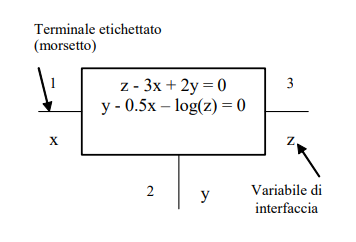
\includegraphics[width=0.5\textwidth]{capitoli/capitolo1/immagini/image1.png}
\end{figure}


\subsection*{Collegamento}
Un collegamento è un arco orientato o non che collega fra loro i morsetti dei componenti circuitali. 
Impedisce l'omogeneità e la continuità alle variabili in corrispondenza dei morsetti. 
Costituisce un'equazione di \textbf{vincolo} fra variabile e interfaccia.
L'insieme dei collegamenti può essere descritto da un grafo opportuno.

\subsection*{Sistema risolvente del circuito}
Il sistema risolvente del circuito è costituito dall'insieme delle equazioni costitutive del componente, equazioni di vincolo, condizioni iniziali e andamenti imposti da cause. 

\subsection*{Risolvere un circuito}
L'obiettivo di risolvere un circuito è calcolare gli andamenti temporali delle variabili di interfaccia. 
Questo è possibile solo se il sistema ammette una soluzione unica ogni istante di tempo.

\subsection*{Due classi di circuiti}
\subsubsection*{Circuiti non direzionali}
\begin{itemize}
    \item La direzione degli scambi è indeterminata.
    \item Non è stabilito un rapporto causa-effetto.
    \item Le variabili di interfaccia dipendono dai componenti del circuito.
    \item La tecnica di soluzione calcola tutte le variabili di interfaccia.
    \begin{figure}[H]
        \centering
        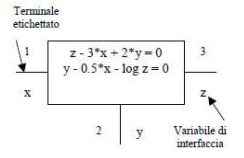
\includegraphics[width=0.5\textwidth]{capitoli/capitolo1/immagini/image2.png}
    \end{figure}
\end{itemize}

\subsubsection*{Circuiti (uni-)direzionali}
\begin{itemize}
    \item La direzione è stabilita a priori.
    \item Il funzionamento è disaccoppiato.
    \item La tecnica di soluzione calcola sequenzialmente le variabili di interfaccia.
    \begin{figure}[H]
        \centering
        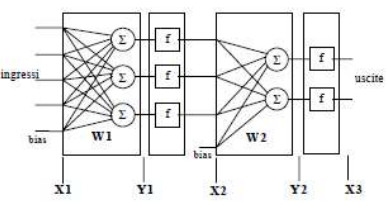
\includegraphics[width=0.7\textwidth]{capitoli/capitolo1/immagini/image3.png}
    \end{figure}
\end{itemize}

\subsection*{Variabili di interfaccia}
Le variabili di interfaccia sono grandezze (segnali) definite sui collegamenti tra componenti, sottoposte a equazioni di vincolo generate dai collegamenti e dalle equazioni dei componenti. 
Tutte le variabili sono funzioni di una o più variabili indipendenti comuni (solitamente il tempo).

\subsection*{Tipi di variabili di interfaccia}
\begin{figure}[H]
    \centering
    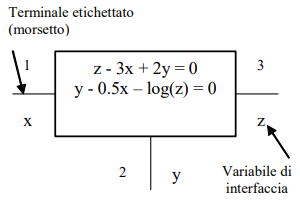
\includegraphics[width=0.7\textwidth]{capitoli/capitolo1/immagini/image4.png}
\end{figure} 
\begin{itemize}
    \item \textbf{A tempo continuo}
    \begin{itemize}
        \item Analogiche.
        \item Riproducono grandezze del mondo fisico.
        \item Hanno un valore per ogni istante \( t \).
        \item A valori reali, limitate, continue.
        \item Possono essere considerate anche a valori complessi, non continue e non limitate.
    \end{itemize}
    \item \textbf{A tempo discreto}
    \begin{itemize}
        \item Digitali.
        \item A valori discreti.
        \item Un solo valore per istanti discreti \( n \).
        \item A valori reali, limitate e continue.
        \item Possono essere considerate anche a valori complessi, non limitate.
    \end{itemize}
\end{itemize}

\section{Circuiti}

\subsection*{Circuiti analogici}
I circuiti analogici sono circuiti con variabili di interfaccia analogiche e relazioni costitutive a tempo continuo.

\subsection*{Circuito a tempo discreto}
Un circuito a tempo discreto è costituito da elementi hardware programmabili via software, con variabili di interfaccia e relazioni costitutive a tempo discreto.

\section{Approccio Circuitale}
\begin{itemize}
    \item Utilizzato per modellare fenomeni fisici diversi.
    \item Modellazione semplice e flessibile.
    \item Applicabile sia a modelli a tempo continuo che a tempo discreto.
    \item Può introdurre approssimazioni.
    \item Il limite è la frequenza e le dimensioni del circuito.
\end{itemize}

\chapter{modello Circuitale}
\section{Modello Circuitale Elettrico}

\subsection*{Equazioni di Maxwell}
Le \textbf{Equazioni di Maxwell} permettono di studiare i fenomeni elettromagnetici e ottenere modellazioni precise del loro funzionamento.

\subsection*{Approccio Circuitale}
L'\textbf{Approccio Circuitale} serve a ottenere un modello semplificato di fenomeni.

\subsection*{Circuiti Elettrici a Costanti Concentrate}
I \textbf{Circuiti Elettrici a Costanti Concentrate} derivano da approssimazioni delle equazioni di Maxwell:

\begin{itemize}
    \item Dimensioni della struttura trascurabili
    \item Velocità di propagazione infinita
    \item Tempo nullo di trasmissione dei fenomeni
\end{itemize}

\textit{È ovviamente necessario verificare la validità delle approssimazioni.}

\begin{figure}[H]
    \centering
    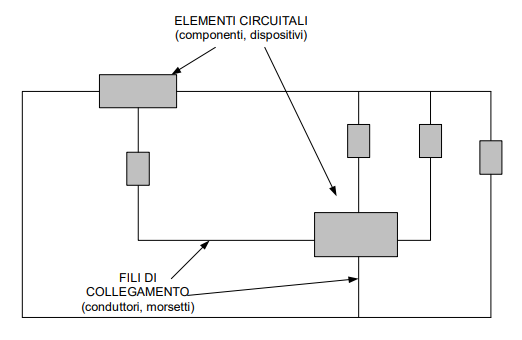
\includegraphics[width=0.7\textwidth]{capitoli/capitolo2/immagini/image1.png}
\end{figure}

\subsection*{Circuito a Costanti Concentrate}
Un \textbf{Circuito a Costanti Concentrate} è una connessione tra elementi ideali privi di dimensioni geometriche e caratterizzati da legami tra tensione e corrente.

\section{Grandezze Elettriche}

\subsection*{Tensione}
La \textbf{Tensione} è definibile tra due morsetti e si misura in \textit{Volt}. È necessario indicare intensità e verso. Il segno negativo indica inversione di polarità.

\subsection*{Corrente}
La \textbf{Corrente} è definibile su un morsetto e si misura in \textit{Ampere}. È necessario indicare intensità e verso. Il segno negativo indica inversione di direzione.

\begin{figure}[H]
    \centering
    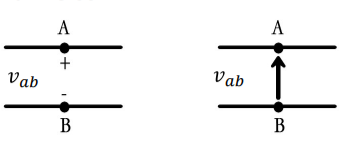
\includegraphics[width=0.7\textwidth]{capitoli/capitolo2/immagini/image2.png}
\end{figure}

\section{Porta Elettrica}

Una \textbf{Porta Elettrica} è costituita da una coppia di morsetti, con la relazione \(i' = i''\).

\subsection*{Grandezze di Porta}
Le grandezze associate alla porta sono \textbf{tensione} e \textbf{corrente}.

\subsection*{Potenza Istantanea}
La potenza istantanea si calcola come:
\[
p(t) = v(t) \cdot i(t) \quad \text{[Watt]}
\]

\subsection*{Versi}
Esistono due versi per la potenza istantanea:

\begin{figure}[H]
    \centering
    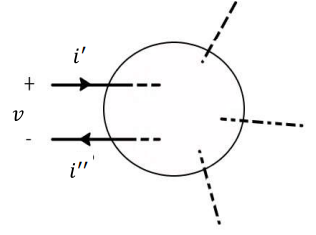
\includegraphics[width=0.7\textwidth]{capitoli/capitolo2/immagini/image3.png}
\end{figure}

\begin{itemize}
    \item \textbf{Porta dell’utilizzatore:} versi coordinati, potenza assorbita > 0.
    \item \textbf{Porta elettrica del generatore:} potenza assorbita < 0, versi non coordinati.
\end{itemize}

\section{Leggi di Kirchhoff}

\subsection*{Prima Legge di Kirchhoff (KLC)}
La somma algebrica delle correnti entranti e uscenti da una superficie chiusa è nulla. La superficie non può tagliare dei componenti, ma solo dei morsetti.

\begin{itemize}
    \item Correnti uscenti → segno +
    \item Correnti entranti → segno -
\end{itemize}

\begin{figure}[H]
    \centering
    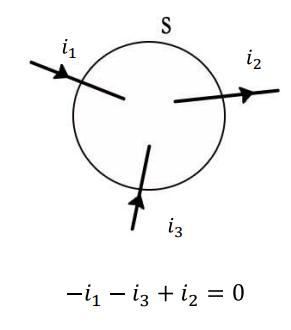
\includegraphics[width=0.7\textwidth]{capitoli/capitolo2/immagini/image4.png}
\end{figure}

\subsection*{Seconda Legge di Kirchhoff}
La somma algebrica delle tensioni lungo una curva chiusa è nulla. La curva chiusa non può tagliare dei componenti, ma solo dei morsetti.

\begin{itemize}
    \item Tensioni senso orario → segno +
    \item Tensioni senso antiorario → segno -
\end{itemize}

\begin{figure}[H]
    \centering
    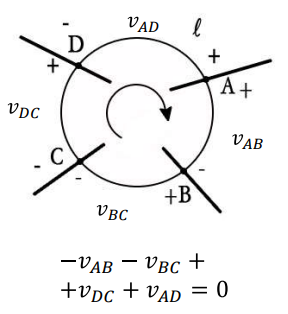
\includegraphics[width=0.7\textwidth]{capitoli/capitolo2/immagini/image5.png}
\end{figure}

\section{Componenti}

Un \textbf{Componente} è costituito da due o più terminali (poli). Un componente con N terminali è detto N-polo. Ad esempio, un bipolo è un componente con due poli.

\subsection*{Bipolo}
Un bipolo ha due morsetti che costituiscono una porta. Le grandezze elettriche sono \(v(t)\) e \(i(t)\). La relazione costitutiva di un bipolo completo è:
\[
f(v(t), i(t), t) = 0
\]
Un bipolo può essere pilotato in tensione o in corrente.

\subsubsection*{Pilotato in Tensione}
Se il bipolo è pilotato in tensione, la relazione è:
\[
i(t) = g v(v(t), t)
\]

\subsubsection*{Pilotato in Corrente}
Se il bipolo è pilotato in corrente, la relazione è:
\[
v(t) = g i(i(t), t)
\]

\subsection*{Potenza Istantanea}
La potenza istantanea per un bipolo è:
\[
p(t) = v(t) \cdot i(t)
\]

\subsection*{Versi Coordinati}
La potenza maggiore di zero viene effettivamente assorbita.

\begin{figure}[h!]
    \centering
    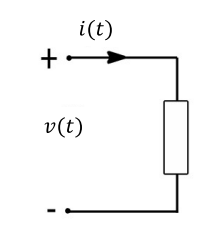
\includegraphics[width=0.7\textwidth]{capitoli/capitolo2/immagini/image6.png}
\end{figure}

\subsection*{Tripolo}
Un tripolo è un componente con tre terminali. La corrente in un tripolo è definita come la somma delle correnti nei terminali:
\[
i(t) = i_1(t) + i_2(t)
\]
Ogni coppia di morsetti può essere considerata come una porta elettrica.

\subsubsection*{2-porte sbilanciato}
Un tripolo può essere modellato come un sistema con due equazioni costitutive che legano le quattro grandezze di porta.

\subsubsection*{Potenza Istantanea}
La potenza istantanea per un tripolo è la somma delle potenze delle due porte:

\begin{figure}[H]
    \centering
    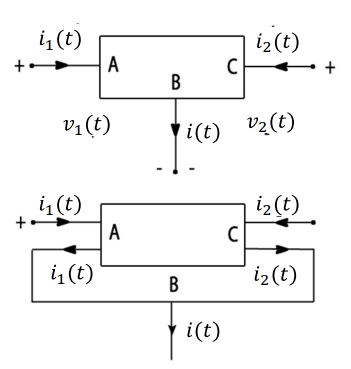
\includegraphics[width=0.7\textwidth]{capitoli/capitolo2/immagini/image7.png}
\end{figure}

\[
p(t) = v_1(t) \cdot i_1(t) + v_2(t) \cdot i_2(t)
\]

\subsection*{Quadripolo}
Un quadripolo è un componente con quattro terminali. La legge di Kirchhoff per le correnti (KLC) non pone vincoli particolari per un quadripolo.

\begin{figure}[H]
    \centering
    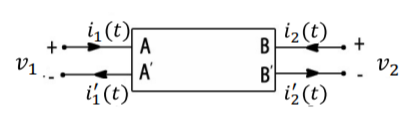
\includegraphics[width=0.7\textwidth]{capitoli/capitolo2/immagini/image8.png}
\end{figure}

\subsubsection*{2-porte Bilanciato}
Nel caso di un quadripolo bilanciato, la potenza istantanea è data da:
\[
p(t) = v_1(t) \cdot i_1(t) + v_2(t) \cdot i_2(t)
\]

\section{Ipotesi Aggiuntive}

\subsection*{Linearità}
Un sistema è lineare se l'effetto è proporzionale alla causa. La linearità permette l'uso del principio di sovrapposizione.
\[
e(t) \to \text{effetto dovuto alla causa } c(t)
\]
\[
a \to \text{costante}
\]

% Relazione tra c(t) e e(t)
\[
\text{*H*}: \text{Se } c(t) \xrightarrow{} e(t) \text{ allora } ac(t) \xrightarrow{} ae(t)
\]

% Conseguenza
\[
\text{*Conseguenza*}: 
\]
\begin{figure}[h!]
    \centering
    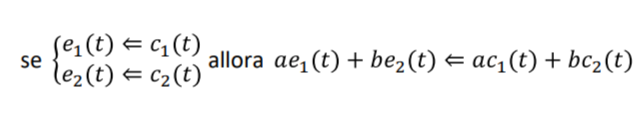
\includegraphics[width=0.7\textwidth]{capitoli/capitolo2/immagini/image9.png}
\end{figure}

\subsection*{Permanenza}
Un sistema è permanente se l'effetto non dipende dall'istante di applicazione della causa:
\[
c(t) \implies e(t) \quad \Rightarrow \quad c(t+t_0) \implies e(t+t_0) \quad \forall t_0 \text{ costante}
\]

\subsection*{Causalità}
Un sistema è causale se, in ogni istante \( t_0 \), l'effetto dipende solo dalla causa per \( t \leq t_0 \).

\begin{figure}[H]
    \centering
    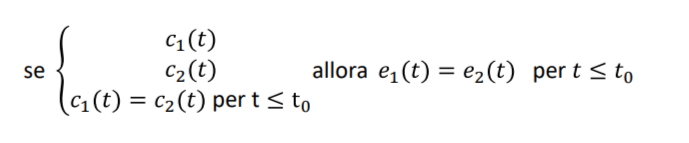
\includegraphics[width=0.7\textwidth]{capitoli/capitolo2/immagini/image10.png}
\end{figure}

\section{Proprietà Notevoli}

Le proprietà come \textbf{linearità}, \textbf{permanenza} e \textbf{causalità} devono essere soddisfatte in ogni sistema.

\subsection*{Reciprocità e Passività}
Le proprietà di reciprocità e passività possono essere verificate in un sistema.

\subsection*{Reciprocità}
La reciprocità implica che l'interazione tra due cause in un circuito non cambia se si scambiano ingresso e uscita.

\begin{figure}[H]
    \centering
    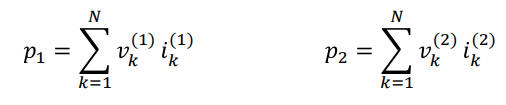
\includegraphics[width=0.7\textwidth]{capitoli/capitolo2/immagini/image11.png}
\end{figure}


\begin{figure}[H]
    \centering
    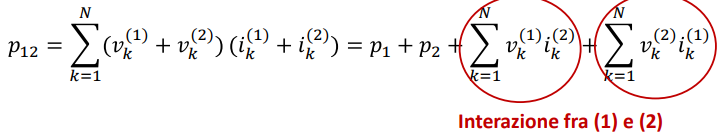
\includegraphics[width=0.7\textwidth]{capitoli/capitolo2/immagini/image12.png}
\end{figure}

\section*{Condizione di reciprocità}

\textbf{Legge di reciprocità di Lorentz}

In due situazioni elettriche diverse, un N-porte è reciproco se vale la condizione precedente.

Dato un componente lineare passivo:

\begin{enumerate}
    \item Si collega un generatore ideale di tensione in A e si considera la corrente di corto circuito in B: \( E_a I_b \)
    \item Si collega un generatore ideale di tensione in B e si considera la corrente di corto circuito in A: \( E_b I_a \)
\end{enumerate}

\textbf{Allora}: 
\[
\frac{E_a}{I_b} = \frac{E_a}{I_a}
\]

\textbf{E se}: 
\[
E_a = E_b \quad \text{e} \quad I_a = I_b 
\]
il comportamento del circuito non cambia scambiando ingresso e uscita.

\textbf{Passività}: L’effetto di una causa di breve durata scompare con il passare del tempo.

- È impossibile fornire energia (o al massimo minore di quella assorbita).

\[
t = -\infty \quad \Rightarrow \quad \text{circuito o componente a riposo}
\]

\subsection*{Passività}
Un sistema è passivo se l'effetto di una causa scivola nel tempo, senza fornire energia.

\section{Componenti Ideali}

\subsection*{Resistore}
Un resistore è misurato in \textit{Ohm} e segue la relazione:
\[
v(t) = R \cdot i(t)
\]

\subsection*{Condensatore}
Un condensatore ha una capacità misurata in \textit{Farad} e segue la relazione:
\[
i(t) = C \frac{d v(t)}{dt}
\]

\section*{Equazione Costitutiva}

\[
v(t) = R i(t) \quad \text{(R costante reale)}
\]

\[
R = \frac{v(t)}{i(t)}
\]

\[
G = \frac{1}{R} = \frac{i(t)}{v(t)} \quad \Rightarrow \quad i(t) = G v(t)
\]

\textbf{Condizione di passività:}

\textbf{Passivo} $\Rightarrow R \geq 0$ (componente reale)

\[
P(t) = R i^2(t) \geq 0 \quad \text{(trasferimento irreversibile di energia)}
\]

Allo zero assoluto è un superconduttore.

\textbf{Attivo} $\Rightarrow R < 0$

\[
P(t) = R i^2(t) < 0 \quad \text{(erogano energia)}
\]

\section*{Condensatore}

Capacità misurata in Farad.

\textbf{Componenti reali} sono caratterizzati dalla tensione di isolamento.

\[
i(t) = C \frac{d v(t)}{dt} \quad \text{(C costante reale)}
\]

\textbf{Passivo} $\Rightarrow C \geq 0$ (componente reale)

\textbf{Attivo} $\Rightarrow C < 0$

Componente con memoria.

\section*{Induttore}

Induttanza misurata in Henry.

\[
v(t) = L \frac{d i(t)}{dt} \quad \text{(L costante reale)}
\]

\textbf{Condizione di passività:}

\textbf{Passivo} $\Rightarrow L \geq 0$

\textbf{Attivo} $\Rightarrow L < 0$

Componente con memoria.

\section*{Generatore Indipendente di Tensione}

Ingresso al circuito.

L'energia può assumere qualsiasi valore.

Componente attivo.

\[
v(t) = V_g(t) \quad \text{(funzione del tempo, eventualmente costante)}
\]

Cortocircuito: $v_g(t) = 0$

\section*{Generatore Indipendente di Corrente}

Ingresso al circuito.

\[
i(t) = i_g(t)
\]

L'energia può assumere qualsiasi valore.

Componente attivo.

Circuito aperto: $i_g(t) = 0$

\section*{Circuiti Equivalenti dei Bipoli Reali}

E' necessario modellare il componente reale considerando altri elementi ideali.

L'inserimento di una resistenza elimina l'assurdo.

\textbf{Resistori in serie}: percorsi dalla stessa corrente $i$.

\textbf{Partitore di tensione}: la tensione si ripartisce su più resistori in maniera proporzionale alle resistenze.

\textbf{Resistori in parallelo}: ai capi hanno la stessa tensione.

\section*{Connessione di Bipoli}

\textbf{Partitore di corrente}: la corrente si ripartisce in maniera inversamente proporzionale alle resistenze.

\section*{Componenti Ideali}

\textbf{2-porte}:

\begin{itemize}
    \item Tripolari o quadrdipolari.
    \item Non sempre hanno un equivalente componente reale.
    \item Utili per circuiti più complessi.
    \item Generatori controllati: elementi attivi, non reciproci, si possono realizzare tutti i 4 tipi da uno solo.
\end{itemize}


\textbf{Nullore}: possono assumere valori qualsiasi, poco realistico, attivo e non reciproco.

\textbf{Trasformatore ideale}: non assorbe potenza, senza perdite, passivo, reciproco.

\textbf{Induttori manualmente accoppiati}: trasferimento reversibile vincolato di energia, componente con memoria.

\textbf{Giratore}: non assorbe potenza, senza perdite, passivo, non reciproco.

\chapter{Fenomeni elettromagnetici}

\section*{Caratteristiche}
\begin{itemize}
    \item \textbf{Grandezze fisiche}
    \begin{figure}[h!]
        \centering
        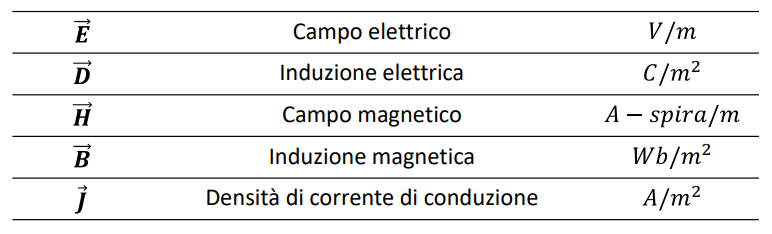
\includegraphics[width=0.7\textwidth]{capitoli/capitolo3/immagini/image1.png}
    \end{figure}
    \begin{itemize}
        \item Vettoriali
        \item Funzione del punto e del tempo
    \end{itemize}

    \item \textbf{Parametri rappresentativi}
    \begin{figure}[h!]
        \centering
        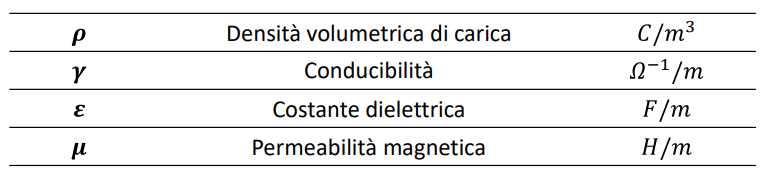
\includegraphics[width=0.7\textwidth]{capitoli/capitolo3/immagini/image2.png}
    \end{figure}

    \vspace{9cm}

    \item \textbf{Equazioni di Maxwell}
    \begin{table}[h]
        \centering
        \renewcommand{\arraystretch}{1.5}
        \begin{tabular}{|l c|}
            \hline
            \textbf{1° Equazione} & \( \nabla \cdot \vec{D} = \rho \) \\
            \hline
            \textbf{2° Equazione} & \( \nabla \cdot \vec{B} = 0 \) \\
            \hline
            \textbf{3° Equazione} & \( \nabla \times \vec{E} = -\frac{\partial \vec{B}}{\partial t} \) \\
            \hline
            \textbf{4° Equazione} & \( \nabla \times \vec{H} = \vec{J} + \frac{\partial \vec{D}}{\partial t} \) \\
            \hline
        \end{tabular}
    \end{table}

    \item \textbf{Relazioni costitutive dei materiali}
    \begin{itemize}
        \item \(\vec{D} = \varepsilon \vec{E} \)
        \item \(\vec{B} = \mu \vec{H} \)
        \item \(\vec{J} = \vec{J_0}+\gamma(\vec{E}-\vec{E_0}) \)
    \end{itemize}
\end{itemize}

\section*{Ipotesi delle costanti concentrate}
\begin{itemize}
    \item Approssimazione del fenomeno elettromagnetico
    \item Dimensioni della struttura trascurabili
    \item Velocit\`a di propagazione \textbf{infinita}
    \item Tempo nullo di trasmissione
    \item Ipotesi valide solo se:
    \begin{itemize}
        \item Tempo di trasmissione \( \ll \) variazioni temporali
        \item Dimensioni spaziali \( \ll \lambda_{min} \)
        \item \( 2 \cdot L_{max} / c \cdot f_{max} \ll 1 \)
    \end{itemize}
\end{itemize}

\section*{Conseguenze delle ipotesi a costanti concentrate}
\begin{itemize}
    \item Velocit\`a di propagazione infinita
    \item Classificazione delle regioni:
    \begin{description}
        \item[\( \varepsilon = 0, \mu = 0 \)] Nessuna energia immagazzinata
        \begin{itemize}
            \item Corrente entrante = corrente uscente
            \item Campo elettrico conservativo
        \end{itemize}
        
        \item[Vuoto ideale]
        \begin{itemize}
            \item Nessuna sollecitazione
            \item \( \sigma = 0 \): non passa corrente
        \end{itemize}

        \vspace{1cm}

        \item[Conduttore ideale]
        \begin{itemize}
            \item \( \sigma \rightarrow \infty \)
            \item Regione equipotenziale
        \end{itemize}

        \item[Resistore]
        \begin{itemize}
            \item \( \sigma \) finita
            \item Dissipazione di potenza
        \end{itemize}

        \item[Generatore indip. di corrente]
        \begin{itemize}
            \item \( \sigma = 0 \)
            \item Trasformazione di energia
        \end{itemize}

        \item[Generatore indip. di tensione]
        \begin{itemize}
            \item \( \sigma \rightarrow \infty \)
            \item Trasformazione di energia
        \end{itemize}

        \item[\( \varepsilon \neq 0, \mu = 0 \): Condensatore]
        \begin{itemize}
            \item Energia elettrica presente
            \item Potenziale definito univocamente
        \end{itemize}

        \item[\( \varepsilon = 0, \mu \neq 0 \): Induttore]
        \begin{itemize}
            \item Energia magnetica presente
            \item Corrente entrante = corrente uscente
        \end{itemize}
    \end{description}
\end{itemize}

\section*{Modello circuitale a costanti concentrate}
\begin{itemize}
    \item Modello composto da regioni tipo:
    \begin{description}
        \item[IA] Vuoto ideale
        \item[IB] Conduttore ideale
        \item[IC] Resistore
        \item[ID] Generatore indip. di corrente
        \item[IE] Generatore indip. di tensione
        \item[II] Condensatore
        \item[III] Induttore
    \end{description}
\end{itemize}

\section*{Leggi di Kirchhoff}
\subsection*{Legge delle correnti (KCL)}
Per ogni superficie chiusa che interseca solo conduttori ideali:
\begin{center}
La somma delle correnti entranti = somma delle correnti uscenti
\end{center}

\subsection*{Legge delle tensioni (KVL)}
Per ogni percorso chiuso che interseca solo conduttori ideali:
\begin{center}
La somma algebrica delle tensioni su un circuito chiuso \`e nulla
\end{center}

\chapter{Segnali e Sistemi a Tempo Discreto}

\section{Segnali a Tempo Discreto}

I segnali a tempo discreto sono rappresentati come $x[n]$, dove $n$ è un numero intero che indica l'indice temporale.

\subsection*{Esempi di segnali a tempo discreto}

\begin{itemize}
    \item \textbf{Impulso unitario} $\delta[n]$: 
    \begin{itemize}
        \item $\delta[n]=1$ se $n = 0$, altrimenti $\delta[n]=0$
        \item Da non confondere con la delta di Dirac
    \end{itemize}
    \item \textbf{Gradino unitario}:
    \begin{itemize}
        \item $u[n]=1$ per $n\geq0$, altrimenti $u[n] = 0$
    \end{itemize}
    \item \textbf{Sequenza esponenziale}:
    \begin{itemize}
        \item $x[n]= Ca^n$, dove $C$ e $a$ sono costanti
        \item Se $a$ è reale $\Rightarrow$ sequenza esponenziale reale
        \item Se $a$ è complesso $\Rightarrow$ sequenza esponenziale complessa
        \item \textbf{Sequenze unilaterali}:
        \begin{itemize}
            \item $x[n]= ca^n u[n]$ (destra)
            \item $x[n]= ca^n u[-n]$ (sinistra)
        \end{itemize}
        \item \textbf{Sequenza a singola frequenza}: $x[n]= ce^{j\omega_0 n}$
        \item \textbf{Segnale sinusoidale}: $x[n]=A\cos(\omega_0n+\varphi)$
    \end{itemize}
\end{itemize}

\section{Domini di Trasformazione}

\subsection*{Trasformata Zeta}
\begin{itemize}
    \item Definizione: $X(z)=\sum\limits_{n=-\infty}^{+\infty} x[n]z^{-n}$
    \item La somma converge solo in una \textbf{Regione di Convergenza (ROC)}
    \item La ROC è fondamentale per:
    \begin{enumerate}
        \item Inversione della trasformata Zeta
        \item Proprietà di causalità e stabilità dei sistemi
    \end{enumerate}
    \item Esempio: $X(z)=\sum\limits_{n=0}^{\infty} a^n z^{-n} \Rightarrow$ converge se $|z| > |a|$
\end{itemize}

\subsection*{Trasformata di Fourier}

\begin{itemize}
    \item Definizione: $X(e^{j\omega})=\sum\limits_{n=-\infty}^{+\infty} x[n]e^{-j\omega n}$
    \item Proprietà: periodica con periodo $2\pi$
    \item Esiste se la ROC della trasformata Z include il cerchio unitario
\end{itemize}

\subsection*{Legame tra Trasformata Z e Fourier}

\begin{itemize}
    \item Relazione: $X(z)|_{z=e^{j\omega}} = X(e^{j\omega})$
\end{itemize}

\section{Sistemi a Tempo Discreto}

\subsection*{Definizione}

Sistemi che operano su $x[n]$ per generare $y[n]$.

\subsection*{Proprietà}
\begin{itemize}
    \item \textbf{Linearità}: somma ponderata delle risposte
    \item \textbf{Stazionarietà (invarianza temporale)}
    \item \textbf{Causalità}: $y[n]$ dipende solo da $x[k]$ con $k\leq n$
    \item \textbf{Stabilità BIBO}: $\sum |h[n]| < \infty$
\end{itemize}

\subsection*{Sistemi LTI (Lineari e Tempo-Invarianti)}

\begin{itemize}
    \item \textbf{Risposta all'impulso} $h[n]$
    \item \textbf{Convoluzione}: $y[n] = \sum\limits_{m=-\infty}^{+\infty} h[m]x[n-m]$
    \item \textbf{Trasformata Z}: $Y(z)=H(z)X(z)$
\end{itemize}

\section{Sistemi a Tempo Continuo}

\subsection*{Trasformata di Fourier}
\begin{itemize}
    \item Definizione: $X(j\Omega)=\int_{-\infty}^{+\infty} x(t)e^{-j\Omega t} dt$
    \item Inversa: $x(t)=\frac{1}{2\pi} \int_{-\infty}^{+\infty} X(j\Omega)e^{j\Omega t} d\Omega$
\end{itemize}

\subsection*{Trasformata di Laplace}
\begin{itemize}
    \item Definizione: $H_a(s)=\int_{-\infty}^{+\infty} h_a(t)e^{-st} dt$
    \item Il sistema è BIBO stabile se tutti i poli sono nel semipiano sinistro: $\text{Re}[s] < 0$
\end{itemize}

\subsection*{Campionamento}

\begin{itemize}
    \item Relazione: $x[n] = x_a(nT)$ con $T>0$
    \item Aliasing se $f_s < 2f_{\text{max}}$
\end{itemize}

\section{Sistemi MIMO}

\begin{itemize}
    \item Matrice di trasferimento $H_{km}(z)$
    \item Modello: $Y(z) = H(z)U(z)$
\end{itemize}

\section{Sistemi LTI: FIR e IIR}

\subsection*{FIR (Finite Impulse Response)}

\begin{itemize}
    \item \textbf{Definizione:}
    
    \[
    H[z] = \sum_{n=0}^{N} h(n) z^{-n}
    \]
    
    dove $N+1$ è la lunghezza del filtro.
    
    \item \textbf{Stabilità:} sempre stabile se $|h(n)| < +\infty$
\end{itemize}

\subsection*{IIR (Infinite Impulse Response)}

\begin{itemize}
    \item \textbf{Definizione:} sistema non FIR
    \item \textbf{Stabilità:} può essere instabile se i poli non sono all'interno del cerchio unitario
\end{itemize}

\subsection*{Strutture per filtri razionali}

Possono essere rappresentati da funzioni razionali:
\section{Sistemi LTI: FIR e IIR}

\subsection*{Strutture per filtri razionali}

Possono essere rappresentati da funzioni razionali:

\[
H(z) = \frac{B(z)}{A(z)}
\]

\[
B(z) = \sum_{n=0}^{N} b_n z^{-n} \quad \text{e} \quad A(z) = \sum_{n=0}^{N} a_n z^{-n}
\]

\textit{Per il filtro FIR} \( A(z) = 1 \).

H(z) può essere descritta da un'equazione alle differenze della forma:

\[
a_0 y(n) = - \sum_{m=1}^{N} a_m y(n-m) + \sum_{m=0}^{N} b_m x(n-m)
\]
\textbf{Forma diretta IIR:}
\begin{figure}[H]
    \centering
    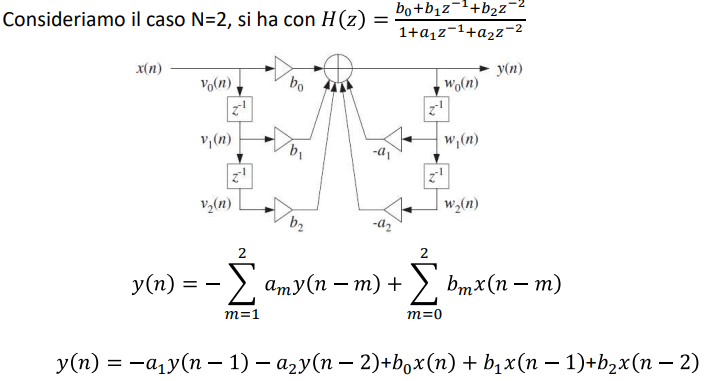
\includegraphics[width=0.7\textwidth]{capitoli/capitolo4/immagini/image1.png}
\end{figure}

\textbf{L'equazione alle differenze} può essere scritta come:

\[
w_0(n) = - a_1 w_1(n) - a_2 w_2(n) + b_0 v_0(n) + b_1 v_1(n) + b_2 v_2(n)
\]

\[
y(n) = w_n(n)
\]
\section{Forma canonica o diretta II (IIR)}

L'equazione della forma canonica diretta II è:

\[
y(n) = (b_0 x(n) + b_1 x(n-1) + b_2 x(n-2)) + (-a_1 y(n-1) - a_2 y(n-2))
\]

Dal momento che le linee di ritardo sono le stesse, non è necessario tenerle separate.
\section{Forma in cascata (IIR)}

\subsection*{Definizione}

La funzione di trasferimento viene espressa come **prodotto di sezioni del secondo ordine (SOS)**:

\[
H(z) = \prod_{i=0}^{K-1} H_i(z)
\]

con ogni \( H_i(z) \) rappresentante una sezione del secondo ordine.

Ogni **funzione di trasferimento razionale** può essere riscritta come prodotto di sezioni del secondo ordine:

\[
H(z) = \frac{b_0 + b_1 z^{-1} + b_2 z^{-2} + \dots + b_M z^{-M}}{1 + a_1 z^{-1} + a_2 z^{-2} + \dots + a_N z^{-N}}
\]

\subsection*{Struttura della Forma in Cascata}

- Ogni **sezione** può essere implementata con una **forma canonica diretta** (o trasposta).
- Convenzionalmente, si utilizza **la forma canonica**.

\subsection*{Segnali di ingresso e uscita}

- **Ingresso del sistema**: il segnale \( x(n) \) entra nella prima sezione.
- **Uscita del sistema**: il segnale in uscita dall'ultima sezione \( y(n) \).
- **Per gli step intermedi**: l’uscita della sezione \( i \) è l’ingresso della sezione \( i+1 \).

\subsection*{Vettore di stato di ogni sezione}

Ogni sezione ha uno **stato interno**:

\[
s_i = [s_{i0}, s_{i1}, s_{i2}]
\]

che rappresenta i **ritardi interni** della sezione.

\subsection*{Equazione alle differenze}

Deriva dalla **forma canonica del secondo ordine**, iterata per tutte le sezioni:

\[
y(n) = -a_1 y(n-1) - a_2 y(n-2) + b_0 x(n) + b_1 x(n-1) + b_2 x(n-2)
\]

\subsection*{Pseudocodice per il calcolo sequenziale}

\[
\begin{aligned}
    x_0 &= x(n) \\
    y_i &= \sum (\text{contributo ritardi e coefficienti}) \\
    x_{i+1} &= y_i \\
    y(n) &= y_{K-1}
\end{aligned}
\]


\section{Assaggio da Forma Diretta/Canonica a Cascata}

La conversione da una **forma diretta** (o canonica) a una **forma in cascata** segue questi passaggi fondamentali:

\begin{enumerate}
    \item **Fattorizzazione** del numeratore e del denominatore nei **polinomi del secondo ordine**.
    \item **Trovare le radici** dei due polinomi.
    \item **Raggruppare in polinomi quadratici**:
    \begin{itemize}
        \item Se \textbf{radici reali}:
        \[
        (1 - \alpha_1 z^{-1} + \alpha_2 z^{-2})
        \]
        \item Se \textbf{radici complesse coniugate}:
        \[
        (1 - \beta_1 z^{-1} + \beta_2 z^{-2})
        \]
    \end{itemize}
\end{enumerate}

Questa forma a cascata è utile per garantire una maggiore **stabilità numerica** e per facilitare l’implementazione pratica dei filtri IIR.

\textbf{Forma diretta FIR:}
\begin{figure}[H]
    \centering
    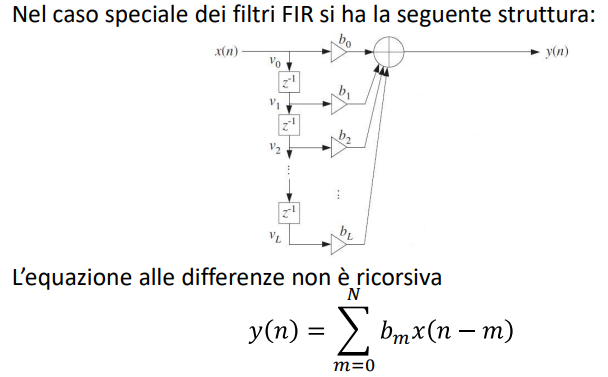
\includegraphics[width=0.7\textwidth]{capitoli/capitolo4/immagini/image2.png}
\end{figure}

\section{Tecniche di filtraggio per filtri IIR}

\subsection{Funzioni delle Librerie Intel}
\begin{itemize}
    \item \textit{Implementazione} suddivisa in:
    \begin{enumerate}
        \item \textbf{Inizializzazione} del filtro
        \item \textbf{Esecuzione del filtraggio}
    \end{enumerate}
    \item Due tipi di \textit{filtri} supportati:
    \begin{enumerate}
        \item \textbf{Filtri di ordine arbitrario} → implementati in \textbf{forma diretta}
        \item \textbf{Filtri biquad} → implementati in \textbf{forma a cascata} (sezioni del secondo ordine)
    \end{enumerate}
\end{itemize}

\subsection{Esempio NU-Tech}
\begin{itemize}
    \item \textbf{Struttura del filtro} dipende dal tipo scelto
    \item \textbf{Inizializzazione richiesta} prima di applicare il filtro
    \item \textbf{Struttura} \texttt{ctx}:
    \begin{itemize}
        \item Contiene i coefficienti \textbf{B} seguiti dai coefficienti \textbf{A} (taps)
    \end{itemize}
\end{itemize}

\subsection{Due Approcci Principali}
\begin{enumerate}
    \item Filtraggio campione per campione (\textbf{Forma Diretta})
    \item Filtraggio a blocchi (\textbf{per segnali lunghi})
\end{enumerate}

\subsection{Forma Diretta e Convoluzione}
Per i sistemi \textbf{LTI}, il filtraggio FIR si basa sulla \textbf{convoluzione}:
\[
    y(n) = \sum_{m=0}^{M} h(m)x(n-m)
\]

\noindent Espressione compatta:
\begin{itemize}
    \item La \textbf{lunghezza finale} del segnale filtrato sarà \(L + M - 1\)
    \item Si basa sul \textbf{concetto di scorrimento} del segnale di input sulla risposta all’impulso
\end{itemize}

\subsection{Funzioni delle Librerie Intel}
\begin{itemize}
    \item Funzione di \textbf{convoluzione} (simile a \texttt{conv} di MATLAB)
    \item Funzioni di \textbf{filtraggio FIR} (inizializzazione come per i filtri IIR, simile a \texttt{filter} di MATLAB)
\end{itemize}

\subsection*{Convoluzione a Blocchi}

La convoluzione a blocchi è utilizzata per il filtraggio real-time di segnali di lunghezza infinita con filtri FIR. Costituisce la base di molte applicazioni in tempo reale.

\medskip

Sono disponibili diversi approcci:

\begin{itemize}
    \item \textbf{OLS (Overlap and Save)}: ad ogni aggiornamento si effettua uno shift del vettore di ingresso verso sinistra, mantenendo solo la parte utile dell'IFFT.
    \item \textbf{OLA (Overlap and Add)}: ad ogni aggiornamento si somma il blocco corrente con quello precedente, dopo aver effettuato uno shift a sinistra.
    \item \textbf{Versione Partizionata}: adatta per blocchi più piccoli (\(L_{\text{BLOCK}} < L_H\)), suddivide il filtro in più blocchi.
\end{itemize}
\textbf{Confronto tra i metodi:}

\begin{table}[H]
\centering
\begin{tabularx}{\textwidth}{|X|X|X|X|}
\hline
\textbf{Metodo} & \textbf{Principio} & \textbf{Vantaggi} & \textbf{Svantaggi} \\
\hline
\textbf{OLS (Overlap and Save)} & Mantiene solo la parte utile dell'IFFT & Risparmio di memoria & Possibile aliasing se non implementato correttamente \\
\hline
\textbf{OLA (Overlap and Add)} & Somma delle finestre successive & Maggiore fedeltà del segnale & Richiede gestione accurata dell'overlap \\
\hline
\textbf{Partizionata} & Suddivide il filtro in blocchi più piccoli & Più efficiente per filtri lunghi & Implementazione più complessa \\
\hline
\end{tabularx}
\caption{Confronto tra approcci per la convoluzione a blocchi}
\end{table}

\section{Convoluzione a Blocchi: OLS (Overlap and Save)}

\textbf{Passaggi principali:}

\begin{enumerate}
    \item \textbf{Shift del buffer} (spostamento di $fs$ campioni)
    \begin{verbatim}
    ippsMove_64f(buffOls + fs, buffOls, fs);
    \end{verbatim}
    
    \item \textbf{Copia dei nuovi $fs$ campioni in fondo al buffer}
    \begin{verbatim}
    ippsCopy_64f((double*)(*Input[0]).DataBuffer, buffOls + fs, fs);
    \end{verbatim}
    
    \item \textbf{Trasformata di Fourier del buffer ($buffOls \to buffOlsF$)}
    \begin{verbatim}
    ippsFFTFwd_RToPack_64f(buffOls, buffOlsF, fftState, 0);
    \end{verbatim}
    
    \item \textbf{FFT dei coefficienti del filtro ($taps \to tapsF$)}
    \begin{verbatim}
    ippsFFTFwd_RToPack_64f_I(tapsF, fftState, 0);
    \end{verbatim}
    
    \item \textbf{Moltiplicazione in frequenza ($buffOlsF \cdot tapsF$)}
    \begin{verbatim}
    ippsMulPack_64f_I(tapsF, buffOlsF, 2fs);
    \end{verbatim}
    
    \item \textbf{Trasformata inversa di Fourier (IFFT)}
    \begin{verbatim}
    ippsFFTInv_PackToR_64f_I(buffOlsF, fftState, 0);
    \end{verbatim}
    
    \item \textbf{Aggiornamento dell'output} (estrazione dei campioni validi)
    \begin{verbatim}
    ippsCopy_64f(buffOlsF + fs, (double*)(*Output[0]).DataBuffer, fs);
    \end{verbatim}
\end{enumerate}

\vspace{3cm}

\section{Convoluzione a Blocchi Partizionata}

\textbf{Passaggi principali:}

\begin{enumerate}
    \item \textbf{Inizializzazione del frame}
    \begin{verbatim}
    CBFunction(this, NUTS_GETFRAME_RATE, 0, &ActualFrameSize);
    in_ols = new double[2*ActualFrameSize];
    memset(in_ols, 0.0, 2*ActualFrameSize * sizeof(double));
    \end{verbatim}
    
    \item \textbf{Copia dei dati di input nel buffer $in\_ols$ e calcolo FFT}
    \begin{verbatim}
    ippsCopy_64f((double*)Input[0]->DataBuffer, in_ols, FrameSize);
    ippsFFTFwd_RToPerm_64f(in_ols, TmpFreqRis, IPP_Spec, NULL);
    \end{verbatim}
    
    \item \textbf{Loop sulla partizione dei coefficienti del filtro}
    \begin{verbatim}
    for(int j = 0; j < ceil(len_taps / FrameSize); j++) {
    ippsCopy_64f(taps + j * FrameSize, taps_cut, FrameSize);
    ippsFFTFwd_RToPerm_64f(taps_cut, fft_taps, IPP_Spec, NULL);
    ippsMulPerm_64f_I(TmpFreqRis, fft_taps, 2 * FrameSize);
    ippsFFTInv_PermToR_64f_I(fft_taps, IPP_Spec, NULL);
    }
    \end{verbatim}
    
    \item \textbf{Gestione del delay per la sovrapposizione delle partizioni}
    \begin{verbatim}
    ippsCopy_64f(fft_taps, delay + j * FrameSize, FrameSize);
    memset(taps_cut, 0.0, FrameSize * sizeof(double));
    memset(fft_taps, 0.0, FrameSize * sizeof(double));
    \end{verbatim}
    
    \item \textbf{Somma con il buffer precedente e aggiornamento dell'output}
    \begin{verbatim}
    ippsAdd_64f_I(delay_old, delay, len_delay_old);
    ippsCopy_64f(delay, (double*)Output[0]->DataBuffer, FrameSize);
    ippsCopy_64f(delay + FrameSize, delay_old, len_delay_old);
    \end{verbatim}
\end{enumerate}





\chapter{DFT e FFT}
\section*{Sequenze Periodiche}

Un \textbf{evento periodico} è un evento che si ripete uguale a se stesso ad ogni intervallo \( N \).

\begin{itemize}
    \item \(\omega_0 = \frac{2\pi}{N}\) è la \textit{pulsazione}.
    \item Non è né quadraticamente né assolutamente sommabile.
    \item È una convoluzione di un periodo con un treno di impulsi di periodo \( N \).
    \item Può essere rappresentato dalla serie discreta di Fourier (DFS).
\end{itemize}

\textbf{Fattore di Twiddle}: \( W_N^{-kn} \).

\section*{Proprietà della DFS}

\subsection*{Linearità}
\[
\sum_{k=0}^{N-1} c_1 X_1[k] + c_2 X_2[k] W_N^{-kn} = c_1 \sum_{k=0}^{N-1} X_1[k] W_N^{-kn} + c_2 \sum_{k=0}^{N-1} X_2[k] W_N^{-kn}
\]

\subsection*{Dualità}
La DFS di una sequenza periodica è anch'essa periodica.

\subsection*{Traslazione nel Tempo}
\[
x[n - m] \leftrightarrow X(e^{j\omega}) e^{-j\omega m}
\]

\subsection*{Traslazione in Frequenza}
\[
x[n] \leftrightarrow X(e^{j(\omega + \Delta \omega)}) 
\]

\subsection*{Simmetria}
\[
X(e^{-j\omega}) = X^*(e^{j\omega})
\]

\section*{Relazione tra DTFT e DFS}

Eseguire la DFS corrisponde a valutare \( X(z) \) su \( N \) punti equispaziati sul cerchio unitario.

La DTFT di una sequenza periodica è il prodotto delle trasformate di Fourier del singolo periodo e del treno di impulsi:

\[
X(e^{j\omega}) = \sum_{n=-\infty}^{+\infty} x[n] e^{-j\omega n}
\]

\section*{Sequenze Periodiche di Durata Finita}

\begin{itemize}
    \item Una \textbf{sequenza periodica} è completamente rappresentata dalla sua \textbf{sequenza DFS}.
    \item Una sequenza \textbf{aperiodica} di lunghezza \( N \) può essere resa \textbf{periodica} replicandola sull'asse \( n \).
    \item La DFS di una sequenza corrisponde alla DTFT campionata \( N \) in frequenze equispaziate.
\end{itemize}

\[
x[n] \leftrightarrow X(e^{j\omega}) \quad \text{con} \quad \omega = \frac{2\pi}{N}k \quad \text{per} \quad n=0, \dots, N-1, \quad k=0, \dots, N-1.
\]

\section*{Campionamento in Frequenza}

\textbf{Obiettivo}: Determinare le condizioni in cui la conoscenza di campioni equispaziati di \( X(e^{j\omega}) \) permette la ricostruzione univoca della sequenza \( x[n] \).

\subsection*{Principali Trasformate}

\begin{itemize}
    \item \textbf{DTFT} (Trasformata Discreta di Fourier Continua):
    \[
    X(e^{j\omega}) = \sum_{n=-\infty}^{+\infty} x[n] e^{-j\omega n}
    \]
    
    \item \textbf{Campionamento della DTFT in N punti}:
    \[
    \bar{X}[k] = X(e^{j \frac{2\pi}{N} k})
    \]

    \item \textbf{DFS inversa} (per una sequenza periodica di periodo \( N \)):
    \[
    \bar{x}[n] = \frac{1}{N} \sum_{k=0}^{N-1} \bar{X}[k] W_N^{-kn}
    \]
\end{itemize}

\section*{Campionamento in Frequenza e Convoluzione}

Sostituendo la DTFT, otteniamo:

\[
\bar{x}[n] = \frac{1}{N} \sum_{m=-\infty}^{+\infty} x[m] \left( \sum_{k=0}^{N-1} W_N^{-k(n-m)} \right)
\]

Si dimostra che:

\[
\sum_{k=0}^{N-1} W_N^{-k(n-m)} = \sum_{r=-\infty}^{+\infty} \delta[n - m + rN]
\]

Quindi:

\[
\bar{x}[n] = x[n] * \sum_{r=-\infty}^{+\infty} \delta[n + rN]
\]

\textbf{Conclusione}: Il campionamento in frequenza della DTFT è equivalente a replicare periodicamente la sequenza nel dominio temporale.

\section{Condizioni per la ricostruzione univoca}

Definiamo:

\[
\tilde{y}[n] = \sum_{r=-\infty}^{+\infty} \delta[n + rN]
\]

La sua \textbf{trasformata discreta} è:

\[
\tilde{Y}[k] = \sum_{n=0}^{N-1} \delta[n] e^{-j \left( \frac{2\pi}{N} \right) k n} = 1 \quad \text{per} \quad k = 0, \dots, N-1
\]

Invertendo la DFS (Trasformata di Fourier Discreta):

\[
\tilde{y}[n] = \frac{1}{N} \sum_{k=0}^{N-1} 1 \cdot W_N^{-kn} = \sum_{r=-\infty}^{+\infty} \delta[n + rN]
\]

\textbf{Conclusione:}

Il \textbf{campionamento in frequenza} della DTFT implica che la sequenza venga \textbf{replicata periodicamente} nel dominio temporale.

Se la sequenza originale è limitata a \(N\) campioni, la sua conoscenza in \(N\) punti equispaziati della DTFT è sufficiente per la ricostruzione univoca.


\section*{Aliasing nel Tempo}

Campionare \( X(e^{j\omega}) \) in \( N \) punti equispaziati sul cerchio unitario equivale ad avere la DFS di una sequenza periodica di periodo \( N \). Questa sequenza periodica si ottiene facendo la convoluzione di \( x[n] \) con un treno di impulsi spaziati di \( N \).

\[
\bar{x}[n] = x[n] * \sum_{r=-\infty}^{+\infty} \delta[n + rN]
\]

\textbf{1° Caso}: Se \( x[n] \) ha durata finita \( \leq N \), può essere ricostruita perfettamente dai suoi \( N \) campioni.

\textbf{2° Caso}: Se \( x[n] \) ha durata maggiore di \( N \), si verifica aliasing temporale.

\section*{Trasformata Discreta di Fourier (DFT)}

Una sequenza aperiodica \( x[n] \) di lunghezza \( N \) può essere completamente rappresentata da \( N \) campioni della sua DTFT. La DFT di una sequenza finita di lunghezza \( N \) è anch'essa di lunghezza \( N \).

\textbf{DFT Diretta}:

\[
X[k] = \sum_{n=0}^{N-1} x[n] W_N^{kn}
\]

\textbf{DFT Inversa}:

\[
x[n] = \frac{1}{N} \sum_{k=0}^{N-1} X[k] W_N^{-kn}
\]

\section{Zero Padding}

\textbf{Obiettivo}: Aumentare la lunghezza della DFT senza alterarne il contenuto informativo.

\subsection{Relazione tra DFT e DTFT}
La \textbf{DFT} di \( x[n] \) è ottenuta campionando la \textbf{DTFT} di \( x[n] \) nei punti:

\[
X[k] = \sum_{n=0}^{N-1} x[n] e^{-j \frac{2\pi}{N} k n}
\]

Per \textbf{ricostruire perfettamente} \( x[n] \), servono \textbf{almeno N campioni} della DTFT per evitare aliasing temporale.

\subsection{Effetto dello Zero Padding}
Si \textbf{aumenta la lunghezza della DFT} a \( M > N \) (maggiore risoluzione in frequenza).
Questo si ottiene \textbf{aggiungendo} \( M - N \) zeri alla fine di \( x[n] \):

\[
x_{padded}[n] = \begin{cases}
x[n] & \text{per} \quad 0 \leq n \leq N-1 \\
0 & \text{per} \quad N \leq n \leq M-1
\end{cases}
\]

La \textbf{DFT non cambia}, ma si ottengono \textbf{più campioni della DTFT}, quindi una \textbf{migliore interpolazione} della risposta in frequenza.

\subsection{Effetti dello Zero Padding}
\begin{itemize}
    \item Aumenta la \textbf{risoluzione in frequenza} (più punti disponibili)
    \item \textbf{Non altera il contenuto in frequenza} (non aggiunge nuove informazioni)
    \item Utile per \textbf{visualizzare meglio} la trasformata
\end{itemize}


\section{Convoluzione di Sequenze Periodiche}

Se \( \tilde{x}_1[n] \) e \( \tilde{x}_2[n] \) sono \textbf{sequenze periodiche di periodo N}, allora:

\subsection{Convoluzione Periodica (Proprietà Commutativa)}
\[
y[n] = \sum_{m=0}^{N-1} \tilde{x}_1[m] \cdot \tilde{x}_2[n-m \, (\text{mod} \, N)]
\]

\subsection{Relazione con la DFS}
\[
\tilde{X}_1[n] \cdot \tilde{X}_2[n] = \mathcal{DFT}\left\{ \tilde{x}_1[n] \cdot \tilde{x}_2[n] \right\}
\]

\subsection{Moltiplicazione punto a punto nel dominio del tempo}
La moltiplicazione punto a punto nel dominio del tempo equivale a una convoluzione nel dominio della DFS:
\[
    \tilde{X}_1[n] \cdot \tilde{X}_2[n] = \sum_{m=0}^{N-1} \tilde{x}_1[m] \cdot \tilde{x}_2[n - m \, (\text{mod} \, N)]
\]

\subsection{Convoluzione Circolare}
\textbf{Definizione}: Identica alla convoluzione periodica, ma gli indici sono considerati \textbf{modulo N}.

Per due sequenze finite di lunghezza \( N \):
\[
    X_1[n] \cdot X_2[n] = \sum_{m=0}^{N-1} x_1[m] \cdot x_2[(n - m) \, (\text{mod} \, N)]
\]

\subsection{Relazione con la DFT}
\[
    X_1[n] \cdot X_2[n]= X_1[k] \cdot X_2[k]
\]

\subsection{Moltiplicazione punto a punto nel tempo}
\[
    X_1[n] \cdot X_2[n] = \sum_{m=0}^{N-1} x_1[m] \cdot x_2[(n - m) \, (\text{mod} \, N)]
\]

\section{Rapporto tra Convoluzione Aperiodica e Circolare}

\subsection*{Caso 1: Sequenze finite di lunghezza \( N \)}
\[
\begin{array}{|c|c|}
\hline
\textbf{Aperiodica} & \textbf{Circolare} \\
\hline
x_1[n] * x_2[n] = \sum_{m=0}^{N-1} x_1[m] \cdot x_2[n-m] & x_1[n] * x_2[n] = \sum_{m=0}^{N-1} x_1[m] \cdot x_2[(n - m) \, (\text{mod} \, N)] \\
\hline
\text{DTFT: } X_1(e^{j\omega}) \cdot X_2(e^{j\omega}) & \text{DFT: } X_1[k] \cdot X_2[k] \\
\hline
\text{Risultato: sequenza aperiodica di lunghezza } 2N-1 & \text{Risultato: sequenza periodica di lunghezza N} \\
\hline
\text{Non coincidono in generale} & \\
\hline
\end{array}
\]

\subsection*{Caso 2: Sequenze di lunghezza diversa}
\begin{itemize}
    \item \textbf{Sequenza aperiodica di lunghezza L}
    \item \textbf{Sequenza aperiodica di lunghezza P < L}
\end{itemize}
\[
\begin{array}{|c|c|}
\hline
\textbf{Aperiodica} & \textbf{Circolare} \\
\hline
x_1[n] * x_2[n] = \sum_{m=0}^{L-1} x_1[m] \cdot x_2[n-m] & x_1[n] * x_2'[n] = \sum_{m=0}^{L-1} x_1[m] \cdot x_2'[(n - m) \, (\text{mod} \, L)] \\
\hline
\text{Risultato: sequenza aperiodica di lunghezza } L + P - 1 & \text{Risultato: sequenza circolare di lunghezza L} \\
\hline
& x_2'[n] \text{ è } x_2[n] \text{ con zero-padding fino a } L-1 \\
\hline
\end{array}
\]

\section{Implementazione della Convoluzione Circolare}
\begin{enumerate}
    \item Si \textbf{forma la sequenza}.
    \item Si \textbf{trasla circolarmente}.
    \item Si \textbf{moltiplica punto a punto}.
\end{enumerate}

\section{Costo Computazionale}

Per una sequenza di lunghezza \( N \):

\begin{itemize}
    \item \textbf{Moltiplicazioni complesse} \( \Rightarrow N^2 \) (equivalente a \( 4N^2 \) operazioni reali)
    \item \textbf{Sommatorie complesse} \( \Rightarrow N(N-1) \) (equivalente a \( N(4N - 2) \) operazioni reali)
\end{itemize}

\textbf{Riduzione del costo computazionale}

\begin{itemize}
    \item \textbf{Algoritmi ottimizzati} per il calcolo della DFT a costo inferiore a \( O(N^2) \)
    \item \textbf{Esempio}: Fast Fourier Transform (FFT)
\end{itemize}


\section{Fast Fourier Transform (FFT)}

L'FFT sfrutta proprietà matematiche per ridurre il numero di operazioni necessarie:

\subsection{Formula della DFT}
\[
X[k] = \sum_{n=0}^{N-1} x[n] \cdot e^{-j \frac{2\pi}{N} k n}
\]

Per ogni campione della DFT:
\begin{itemize}
    \item \textbf{Moltiplicazioni complesse}: \( N \)
    \item \textbf{Somme complesse}: \( N-1 \)
\end{itemize}

Per calcolare \( N \) campioni:
\begin{itemize}
    \item Complessità totale: \( O(N^2) \) \quad \text{(ALTA!)}
\end{itemize}

\subsection{\texorpdfstring{Ottimizzazioni basate sulle Proprietà di \( W_N \)}{Ottimizzazioni basate sulle Proprietà di W\_N}}


\begin{itemize}
    \item \textbf{Simmetria}
    \item \textbf{Periodicità}
\end{itemize}

\section{Radix-2 Decimation In Time (DIT) FFT}

\textbf{Idea (Cooley-Tukey 1965)}

\begin{itemize}
    \item Si suddivide la sequenza \( x[n] \) in due sottosequenze di lunghezza \( N/2 \):
    \begin{itemize}
        \item Campioni \textbf{con indice pari}
        \item Campioni \textbf{con indice dispari}
    \end{itemize}
    \item Si calcola la \textbf{DFT totale} componendo opportunamente le \textbf{DFT delle sottosequenze}.
\end{itemize}

\textbf{Scomposizione della DFT}

\[
X[k] = \sum_{m=0}^{N/2-1} x[2m] W_{N/2}^{km} + W_N^k \sum_{m=0}^{N/2-1} x[2m+1] W_{N/2}^{km}
\]

La DFT a \( N \) punti si scompone in due DFT a \( N/2 \) punti più combinazioni di dati.

\textbf{Algoritmo Iterativo}

\begin{itemize}
    \item Se \( N \) è una potenza di 2, l'algoritmo si applica ricorsivamente fino alla DFT di 2 punti.
    \item \textbf{Numero di stadi}: \( M = \log_2(N) \)
    \item \textbf{Numero totale di "butterfly" per stadio}: \( N/2 \)
\end{itemize}

\textbf{Esempio per \( N=8 \):}

\[
N = 2^3 \Rightarrow 3 \text{ stadi}: \quad \text{DFT 8 punti} \rightarrow \text{DFT 4 punti} \rightarrow \text{DFT 2 punti}
\]
\section*{Varianti dell'algoritmo DIT}

\begin{enumerate}
    \item \textbf{DIT Canonica}
    \begin{itemize}
        \item Ingresso: \textbf{bit-reversed order}
        \item Uscita: \textbf{ordine normale}
        \item \textbf{"In-place"}
    \end{itemize}
    \item \textbf{DIT Alternativa}
    \begin{itemize}
        \item Ingresso: \textbf{ordine normale}
        \item Uscita: \textbf{bit-reversed order}
        \item \textbf{"In-place"}
    \end{itemize}
    \item \textbf{DIT Sequenziale}
    \begin{itemize}
        \item Indici normali in ogni stadio
        \item Non \textbf{in-place} (più complesso)
    \end{itemize}
\end{enumerate}

\section*{Radix-2 Decimation In Frequency (DIF) FFT}

\textbf{Idea:}

La sequenza in ingresso viene divisa in due sottosequenze:
\begin{itemize}
    \item Campioni con indice pari
    \item Campioni con indice dispari
\end{itemize}

Si calcolano separatamente e poi si combinano in uscita.

\section*{Scomposizione della DFT}

\begin{itemize}
    \item Per i campioni \textbf{pari}:
    \[
    X[2m] = \sum_{n=0}^{N/2-1} \left[ x[n] + x[n+N/2] \right] W_{N/2}^{nm}
    \]
    \item Per i campioni \textbf{dispari}:
    \[
    X[2m+1] = \sum_{n=0}^{N/2-1} \left[ x[n] - x[n+N/2] \right] W_{N/2}^{nm} W_N^n
    \]
\end{itemize}

\section*{Algoritmo Iterativo}

\begin{itemize}
    \item Se \( N = 2^M \), si applica ricorsivamente fino a ottenere \textbf{solo DFT a 2 punti}.
    \item \textbf{Numero di stadi}: 
    \[
    M = \log_2 (N)
    \]
    \item \textbf{Numero di "butterfly" per stadio}: \( \frac{N}{2} \)
\end{itemize}

\section*{Butterfly DIF}

\begin{itemize}
    \item Struttura simile a DIT, ma con \textbf{dati e flussi invertiti}.
    \item \textbf{"In-place"} possibile con un solo array di memoria.
\end{itemize}
\section*{Differenze tra DIT e DIF}

\begin{center}
\begin{tabular}{|c|c|c|}
\hline
\textbf{Caratteristica} & \textbf{DIT (Decimation In Time)} & \textbf{DIF (Decimation In Frequency)} \\
\hline
Scomposizione & Sui \textbf{campioni di ingresso} & Sui \textbf{coefficienti di uscita} \\
\hline
Bit-Reversal & \textbf{Ingresso in bit-reversed order} & \textbf{Uscita in bit-reversed order} \\
\hline
Ordine dei W & Normale & Bit-reversed \\
\hline
Algoritmo & \textbf{Top-down} & \textbf{Bottom-up} \\
\hline
\end{tabular}
\end{center}

\section*{Radix-2 Decimation in Time (DIT) FFT}

\textbf{Principio $\rightarrow$} Si scompone la sequenza \( x[n] \) in due sottosequenze (pari e dispari).

\subsection*{Procedura}
\begin{enumerate}
    \item \textbf{Scomposizione ricorsiva} fino a ottenere DFT di lunghezza 2.
    \item \textbf{Combinazione dei risultati} con operazioni butterfly.
    \item \textbf{Bit-reversal} sugli indici in ingresso o uscita.
\end{enumerate}

\section*{Struttura della DIT FFT}

\textbf{Ingresso}: Ordinamento \textbf{bit-reversed}

\textbf{Uscita}: Ordinamento normale

\section*{Butterfly}
\[
X[k] = X'[k] + W_N^k X''[k]
\]

\section*{Computazione in-place}
Un unico array aggiornato a ogni stadio.
\section*{DIT Canonica}

\begin{itemize}
    \item \textbf{Input}: Bit-reversed
    \item \textbf{Output}: Normale
    \item \textbf{Coefficienti W}: Normali
\end{itemize}

\section*{DIT Alternativa}

\begin{itemize}
    \item \textbf{Input}: Normale
    \item \textbf{Output}: Bit-reversed
    \item \textbf{Coefficienti W}: Bit-reversed
\end{itemize}

\section*{DIT Sequenziale}

\begin{itemize}
    \item Indici normali a ogni stadio
    \item \textbf{Non in-place} (maggior uso di memoria)
\end{itemize}

\section*{Struttura della DIF FFT}

\begin{itemize}
    \item \textbf{Ingresso}: Ordinamento normale
    \item \textbf{Uscita}: Ordinamento \textbf{bit-reversed}
\end{itemize}

\section*{Butterfly}
\[
X[k] = X_e[k] + W_N^k X_o[k]
\]

Computazione in-place

\section*{DIF Canonica}

\begin{itemize}
    \item \textbf{Input}: Normale
    \item \textbf{Output}: Bit-reversed
    \item \textbf{Coefficienti W}: Normali
\end{itemize}

\section*{DIF Alternativa}

\begin{itemize}
    \item \textbf{Input}: Bit-reversed
    \item \textbf{Output}: Normale
    \item \textbf{Coefficienti W}: Bit-reversed
\end{itemize}

\section*{DIF Sequenziale}

\begin{itemize}
    \item Indici normali a ogni stadio
    \item \textbf{Non in-place}
\end{itemize}

\section*{Confronto DIT vs DIF}

\begin{center}
\begin{tabular}{|c|c|c|}
\hline
\textbf{Caratteristica} & \textbf{DIT FFT} & \textbf{DIF FFT} \\
\hline
\textbf{Divisione} & Ingresso (x[n]) & Uscita (X[k]) \\
\hline
\textbf{Input} & Bit-reversed & Normale \\
\hline
\textbf{Output} & Normale & Bit-reversed \\
\hline
\textbf{Computazione} & Bottom-up & Top-down \\
\hline
\textbf{Uso memoria} & In-place & In-place \\
\hline
\end{tabular}
\end{center}

\section*{Costo Computazionale}

\begin{itemize}
    \item \textbf{Butterfly}: 1 prodotto complesso + 2 somme complesse.
    \item \textbf{N punti}: N/2 butterfly per stadio.
    \item \textbf{FFT a N punti} ($N = 2^M$): \textbf{M stadi}.
\end{itemize}

\section*{Confronto DFT vs FFT}

\begin{itemize}
    \item \textbf{DFT classica}: O($N^2$)
    \item \textbf{FFT radix-2}: O($N \log N$)
\end{itemize}

\section*{Vantaggi della FFT}

\begin{itemize}
    \item \textbf{Enorme riduzione dei calcoli} rispetto alla DFT.
    \item \textbf{Hardware ottimizzato}: pipeline, unità parallele.
    \item \textbf{Utilizzata in DSP, compressione, imaging}.
\end{itemize}

\section*{Problema principale}

\begin{itemize}
    \item \textbf{Precisione finita nei calcoli numerici.}
\end{itemize}

\section*{Categorie principali di algoritmi FFT}

Gli \textbf{algoritmi FFT} sono stati sviluppati per velocizzare il calcolo della Trasformata Discreta di Fourier (DFT).

\subsection*{Categorie}

\begin{itemize}
    \item \textbf{Radix-M FFT (CFA – Common Factor Algorithm)}:
    \begin{itemize}
        \item $N$ deve essere una potenza di $M$. Il caso più diffuso è il \textbf{radix-2}.
        \item Altri esempi includono \textbf{radix-4} o \textbf{radix-8}, che riducono il numero di operazioni richieste.
    \end{itemize}

    \item \textbf{Mixed Radix FFT}:
    \begin{itemize}
        \item Scompone $N$ come un prodotto di fattori diversi (tipicamente 2, 3, 4 o 8).
        \item Ogni stadio dell'algoritmo utilizza un radix differente, migliorando l’efficienza del calcolo rispetto all’approccio standard.
    \end{itemize}

    \item \textbf{Prime Factor FFT (PFA – Prime Factor Algorithm)}:
    \begin{itemize}
        \item $N$ viene scomposto in fattori primi tra loro.
        \item Riduce ulteriormente il numero di moltiplicazioni rispetto alla Mixed Radix FFT.
    \end{itemize}

    \item \textbf{Algoritmo di Winograd}:
    \begin{itemize}
        \item Sfrutta una struttura matematica per trasformare la FFT monodimensionale in una FFT bidimensionale.
        \item Il costo computazionale complessivo è $O(N \log_2 N)$.
        \item Riduce il numero di moltiplicazioni a $O(N)$, seppur aumentando il numero di somme da effettuare.
    \end{itemize}
\end{itemize}

\section*{Utilizzi}

\begin{itemize}
    \item \textbf{Progettazione di filtri FIR}: La trasformata inversa di Fourier (IFFT) viene utilizzata per ottenere il filtro desiderato a partire da una griglia di punti in frequenza.
    \item \textbf{Calcolo della convoluzione e della correlazione}: La FFT permette di eseguire queste operazioni in maniera molto più efficiente rispetto ai metodi tradizionali.
    \item \textbf{Stima spettrale}: Viene sfruttata la relazione tra la DFT e la Trasformata di Fourier Discreta Tempo-Variabile (DTFT) per analizzare segnali di durata finita.
    \item \textbf{Riconoscimento vocale e sistemi radar}: Questi settori utilizzano la FFT per analizzare segnali il cui contenuto spettrale cambia nel tempo.
\end{itemize}

\textbf{Problema critico} → \textbf{Precisione finita}, poiché i calcoli numerici possono introdurre errori dovuti alla rappresentazione discreta dei numeri in hardware.

\textbf{Elaborazione numerica dei segnali (DSP)}: La FFT continua a essere una delle tecniche più utilizzate in innumerevoli applicazioni tecnologiche.

\section*{Calcolo della Convoluzione e della Correlazione con la FFT}

\subsection*{Convoluzione Aperiodica e FFT}

Per due sequenze di lunghezza \( L \) e \( P \), la convoluzione aperiodica può essere calcolata tramite una convoluzione ciclica di \( L+P-1 \) punti. Per sfruttare l'efficienza della FFT, si utilizza lo \textbf{zero-padding} fino alla lunghezza \( L+P-1 \).

\subsection*{Formula della Convoluzione}

La convoluzione aperiodica di due segnali \( x_1[n] \) e \( x_2[n] \) è definita come:

\[
x_1[n] * x_2[n] = \sum_{m=-\infty}^{+\infty} x_1[m] \cdot x_2[n-m]
\]

Questa relazione nel dominio della trasformata diventa:

\[
X_1(e^{j\omega}) \cdot X_2(e^{j\omega})
\]

\subsection*{Schema del Calcolo della Convoluzione con la FFT}

\begin{enumerate}
    \item \textbf{Zero-padding} delle sequenze fino alla lunghezza \( L+P-1 \).
    \item \textbf{Calcolo della FFT} delle sequenze con la stessa lunghezza.
    \item \textbf{Moltiplicazione} delle FFT ottenute.
    \item \textbf{Calcolo della IFFT} per ottenere la convoluzione.
\end{enumerate}

\subsection*{Formula della Correlazione}

La correlazione tra due segnali è definita come:

\[
x_1[n] * x_2[-n] = \sum_{m=-\infty}^{+\infty} x_1[m] \cdot x_2[n+m]
\]

E nel dominio della trasformata diventa:

\[
X_1(e^{j\omega}) \cdot X_2^*(e^{j\omega})
\]

dove \( X_2^* \) è il complesso coniugato della FFT di \( x_2[n] \).

\subsection*{Schema del Calcolo della Correlazione con la FFT}

\begin{enumerate}
    \item \textbf{Zero-padding} delle sequenze fino alla lunghezza \( L+P-1 \).
    \item \textbf{Calcolo della FFT} delle sequenze.
    \item \textbf{Moltiplicazione della FFT di \( x_1[n] \)} con il coniugato complesso della FFT di \( x_2[n] \).
    \item \textbf{Calcolo della IFFT} per ottenere la correlazione.
\end{enumerate}

\subsection*{Ottimizzazioni e Speed-up}

\begin{itemize}
    \item \textbf{Bit-Reversing Ottimizzato:} Si può evitare il bit-reversing usando un algoritmo \textbf{DIF diretto} per la FFT e \textbf{DIT inverso} per la IFFT.
    \item \textbf{Calcolo di DFT in parallelo:} È possibile calcolare \textbf{due DFT di sequenze reali contemporaneamente}, sfruttando la proprietà della FFT per segnali reali.
\end{itemize}

\subsection*{Se una delle Sequenze ha Durata Molto Lunga (Infinita)}

\begin{itemize}
    \item \textbf{Overlap and Add:} Si decompone \( x[n] \) in blocchi senza sovrapposizione.
    \item \textbf{Overlap and Save:} Si decompone \( x[n] \) in blocchi con sovrapposizione di \( P-1 \) punti, calcolando la convoluzione circolare di ogni blocco (FFT a \( L \) punti).
\end{itemize}



\chapter{Sistemi LTI con funzione di trasferimento razionale}

La funzione di trasferimento di un sistema LTI è data da:

\[
H(z) = \frac{B(z)}{A(z)}
\]

\subsection*{Risposta in frequenza}

La risposta in frequenza di un filtro è:

\[
H(e^{j\omega}) = |H(e^{j\omega})| e^{j\phi(\omega)}
\]

\subsection*{Ritardo di gruppo}

Il ritardo di gruppo è dato da:

\[
\tau(\omega) = -\frac{d\phi(\omega)}{d\omega}
\]

\section{Classificazione dei Filtri Digitali}

\subsection*{Filtri a Coefficienti Reali}

- La risposta in frequenza \( H(e^{j\omega}) \) è \textbf{pari}, la fase \( \phi(\omega) \) è \textbf{dispari}.

\subsubsection*{Esempio}

Un esempio di filtro con coefficienti reali è dato da:

\[
H(z) = 1 - a z^{-1}
\]

\subsection*{Filtri a Fase Lineare}

La risposta in frequenza di un filtro a fase lineare è:

\[
H(e^{j\omega}) = c e^{-jK\omega} H_R(\omega)
\]

dove la fase è lineare.

\subsubsection*{Tipi di Filtri a Fase Lineare}

- \textbf{Simmetrico}: fase lineare.
- \textbf{Antisimmetrico}: non adatto a filtri passa-basso o passa-alto.

\section{Specifiche di Progetto}

\subsection*{Banda Passante}

La banda passante è definita come:

\[
0 \leq \omega \leq \omega_p
\]

\subsection*{Banda Oscura}

La banda oscura è definita come:

\[
\omega_s \leq \omega \leq \pi
\]

\subsection*{Zona di Transizione}

La zona di transizione è compresa tra:

\[
\omega_s \quad \text{e} \quad \omega_p
\]

\subsection*{Ampiezza Normalizzata}

L'ampiezza normalizzata è data dalla divisione per:

\[
(1 + \delta_1)
\]

\section{Progetto di Filtri FIR}

\subsection*{Scelta tra FIR e IIR}

- I filtri FIR hanno fase lineare ma un costo computazionale maggiore.
- I filtri IIR sono più efficienti in termini di ordine, ma hanno fase non lineare.

\subsection*{Metodi di Progettazione FIR}

1. \textbf{Windowing}: semplice, ma non ottimizzato.
2. \textbf{Least Square}: minimizza l'errore in frequenza.
3. \textbf{Equiripple}: distribuisce uniformemente l'errore.

\subsubsection*{Metodo Windowing}

Il metodo di windowing prevede il troncamento della risposta impulsiva con una finestra:

- Rettangolare (troncamento semplice).
- Hamming, Blackman, Kaiser (miglior controllo).
- \textbf{Fenomeno di Gibbs}: ripple nella banda passante.

\subsubsection*{Metodo Eigenfilter}

Il metodo eigenfilter minimizza l'errore in banda passante e oscura utilizzando gli autovettori di una matrice.

\subsubsection*{Metodo Equiripple}

L'algoritmo di Parks-McClellan è utilizzato per minimizzare il massimo errore.

\section{Progetto di Filtri IIR}

\subsection*{Trasformazione Bilineare}

1. Progettare il filtro analogico \( H_a(s) \).
2. Applicare la trasformazione bilineare:

\[
s = \frac{1 - z^{-1}}{1 + z^{-1}}
\]

3. Ottenere il filtro digitale \( H(z) \).

\subsection*{Tipologie di Filtri IIR}

1. \textbf{Butterworth}: risposta piatta, transizione lenta.
2. \textbf{Chebyshev I}: banda passante equiripple, banda oscura monotona.
3. \textbf{Chebyshev II}: banda passante monotona, banda oscura equiripple.
4. \textbf{Ellittico}: equiripple in entrambe le bande, transizione più veloce.

\section{Filtri Passa-Tutto}

I filtri passa-tutto mantengono il modulo costante e modificano solo la fase.

\subsection*{Proprietà dei Filtri Passa-Tutto}

- Coppie coniugate reciproche di poli e zeri.
- L'energia di uscita è uguale all'energia di ingresso.



\chapter{Introduzione al Suono e Temperamento Musicale}
\section{Suono e Qualità del Suono}

Il suono è costituito da \textbf{vibrazioni} che vengono trasmesse al nostro orecchio tramite un fluido.

\subsection*{Qualità del Suono}

La qualità del suono dipende da vari fattori, tra cui:

\begin{itemize}
    \item \textbf{Altezza}
    \item \textbf{Intensità}
    \item \textbf{Timbro}
    \item \textbf{Durata}
\end{itemize}

\subsection*{Unità di Misura}

L'unità di misura della frequenza del suono è il \textbf{Hertz} (Hz).

\section{Notazione Musicale}

La notazione musicale può essere divisa in due categorie:

\begin{itemize}
    \item \textbf{Notazione assoluta}
    \item \textbf{Codifica relativa}
\end{itemize}

Questa notazione è utilizzata per scrivere, leggere e scambiare la musica in maniera univoca.

\subsection*{Nomi delle Note}

\begin{itemize}
    \item \textbf{Latino}: Do/Ut, Re, Mi, Fa, Sol, La, Si
    \item \textbf{Inglese}: C, D, E, F, G, A, B
    \item \textbf{Alterazioni}: Sharp, Flat, Natural
\end{itemize}

\subsection*{Ottava}

L'ottava è costituita dalla sequenza:

\[
C, C\#, D, D\#, E, F, G, G\#, A, A\#, B, C'
\]

Poi la sequenza si ripete.

\subsection*{Intonazione}

L'intonazione standard è di 440 Hz.

\section{Temperamento Musicale}

Il \textbf{temperamento} si riferisce al rapporto di frequenze relative agli intervalli musicali.

\subsection*{Temperamento Pitagorico}

Il temperamento pitagorico si basa su due principi fondamentali:

\begin{itemize}
    \item \textbf{Ottava}: rapporto di frequenza di \( 2:1 \)
    \item \textbf{Quinta giusta}: rapporto di frequenza di \( 3:2 \)
\end{itemize}

Seguendo il \textbf{circolo delle quinte} (C $\rightarrow$ G $\rightarrow$ D $\rightarrow$ A $\rightarrow$ E $\rightarrow$ ...), dopo 12 quinte si torna a C, ma il rapporto risultante è:

\[
\left(\frac{3}{2}\right)^{12} \approx 129.75
\]

Mentre 7 ottave corrispondono a:

\[
2^7 = 128
\]

Questa discrepanza è nota come \textbf{comma pitagorico}.

\subsubsection*{Soluzione di Pitagora}

Pitagora ha proposto la seguente soluzione:

\begin{itemize}
    \item Mantenere le \textbf{quinte giuste} (3:2) e le \textbf{quarte giuste} (4:3)
    \item Derivare le altre note dal circolo delle quinte e riportarle all'ottava originale
\end{itemize}

In questo modo si ottengono \textbf{intervalli diseguali}, creando difficoltà nell'intonazione in alcune tonalità.

\subsection*{Temperamento Equabile}

Il \textbf{temperamento equabile} è stato sviluppato per risolvere il problema degli intervalli diseguali. In questo sistema, l'ottava è divisa in \textbf{12 intervalli uguali}. 

\begin{itemize}
    \item L'ottava è sempre \( 2:1 \), ma il \textbf{semitono temperato} è calcolato come la dodicesima radice di 2:

    \[
    \sqrt[12]{2} \approx 1.05946
    \]

    \item Questo sistema permette di avere \textbf{tutti gli intervalli identici}, rendendo possibile suonare in qualsiasi tonalità senza dissonanze evidenti.
\end{itemize}

\section{Trasposizione}

\subsection*{Temperamento Equabile}

Nel temperamento equabile, è possibile fare uno "shift" di \( N \) semitoni, in alto o in basso, senza alterare il rapporto di frequenze tra gli intervalli.

\subsection*{Temperamento Pitagorico}

Nel temperamento pitagorico (e in generale nei temperamenti non equabili), questa proprietà non è vera. Una melodia trasposta suonerà in maniera molto differente.

\section{Tempo e Durata}

Il tempo e la durata sono mappati in un tempo relativo, che viene misurato dal valore del metronomo, solitamente indicato come \textbf{BPM} (battiti per minuto).

\subsection*{Battute e Raggruppamenti}

I battiti sono raggruppati in \textbf{battute}.



\chapter{Introduzione al Protocollo MIDI}

\section{MIDI: Protocollo Musical Instruments Digital Interface}

Il protocollo MIDI è un sistema per la comunicazione tra dispositivi musicali digitali. È un protocollo \textbf{seriale}.

\begin{figure}[h!]
    \centering
    %\includegraphics[width=0.7\textwidth]{Screenshot_2025-03-20_092820.png}
    \caption{Esempio di trasmissione MIDI}
\end{figure}

I dati vengono trasmessi con bit di \textbf{start} e di \textbf{stop}.

\subsection*{Tipi di Byte}

I byte trasmessi possono essere di due tipi:

\begin{itemize}
    \item \textbf{Byte di stato}: MSbit = 1
    \item \textbf{Byte di dati}: MSbit = 0
\end{itemize}

\subsection*{Caratteristiche Generali}

\begin{itemize}
    \item Non c'è collegamento in rete.
    \item Ogni cavo MIDI può trasmettere i dati attraverso \textbf{16 canali}.
    \item I dispositivi possono essere collegati in cascata.
\end{itemize}

\section{Tipi di Messaggi MIDI}

I messaggi MIDI possono essere classificati come segue:

\subsection*{1. Messaggi a 2 byte e 3 byte}

Questi messaggi contengono:

\begin{itemize}
    \item \textbf{Status Byte}
        \begin{itemize}
            \item \textbf{MSB nibble} (3 bit): indica il tipo di messaggio.
            \item \textbf{LSB nibble} (4 bit): indica il canale (0-15, che corrisponde a 1-16 in notazione musicale).
        \end{itemize}
    \item \textbf{Data Byte 1}: contiene informazioni come la nota suonata.
    \item \textbf{Data Byte 2}: contiene altre informazioni come la velocità (velocity).
\end{itemize}

\subsection*{2. Messaggi di Control Change (CC)}

Formato:

\[
0xBi \ 0xCC \ 0xVV
\]

\begin{itemize}
    \item `0xB`: Indica un messaggio di Control Change.
    \item `i`: Indica il canale MIDI (0-15, cioè 1-16 in notazione musicale).
    \item `0xCC`: Numero del controllo.
    \item `0xVV`: Valore assegnato al controllo.
\end{itemize}

\subsection*{3. Messaggi di Program Change}

Utilizzati per cambiare rapidamente preset o patch di strumenti digitali.

Formato base:

\[
0xCi \ 0xPP
\]

\begin{itemize}
    \item `0xC`: Indica un messaggio di Program Change.
    \item `i`: Canale MIDI.
    \item `0xPP`: Numero del preset (da 0 a 127).
\end{itemize}

Per superare il limite di 128 preset, si usano due messaggi di Control Change:

\begin{itemize}
    \item \textbf{MSB Bank Select}: \( 0xBi \ 0x00 \ 0xBB \)
    \item \textbf{LSB Bank Select (opzionale)}: \( 0xBi \ 0x20 \ 0xbb \)
    \item \textbf{Program Change}: \( 0xCi \ 0xPP \)
\end{itemize}

\subsection*{4. Messaggi Speciali MIDI}

\begin{itemize}
    \item \textbf{Pitch Bend}: Permette di variare l’intonazione di una nota in modo continuo.
    \item \textbf{NRPN (Non-Registered Parameter Number)}: Trasmette parametri ad alta risoluzione (fino a 14 bit).
\end{itemize}

\subsubsection*{Formato di NRPN}

\begin{itemize}
    \item `CC 0x63 0xPP`: MSB del parametro.
    \item `CC 0x62 0xpp`: LSB del parametro.
    \item `CC 0x06 0xVV`: MSB del valore.
    \item (Opzionale) `CC 0x26 0xvv`: LSB del valore.
\end{itemize}

\subsection*{5. Messaggi System Exclusive (Sysex)}

Messaggi personalizzati di lunghezza arbitraria, definiti dal produttore.

Formato:

\[
0xF0 \ \text{<ID produttore>} \ \text{<payload>} \ 0xF7
\]

\subsection*{6. Messaggi System Realtime}

Gestiscono il sincronismo e il controllo globale del sistema MIDI.

\begin{itemize}
    \item \textbf{MIDI Clock}: `0xF8` (24 pulse = 1 quarto).
    \item \textbf{Start sequenza}: `0xFA`.
    \item \textbf{Continue sequenza}: `0xFB`.
    \item \textbf{Stop sequenza}: `0xFC`.
    \item \textbf{Active Sensing}: `0xFE`.
\end{itemize}

\subsection*{7. Messaggi di Sistema (System Common CC)}

Comandi per il controllo generale del sistema MIDI.

\begin{itemize}
    \item \textbf{All Sounds OFF}: `0xBi 0x78 0x00`.
    \item \textbf{All Notes OFF}: `0xBi 0x7B 0x00`.
    \item \textbf{Reset All Controllers}: `0xBi 0x79 0x00`.
    \item \textbf{Local Control ON/OFF}: `0xBi 0x7A 0xVV`.
\end{itemize}

\section*{Estensioni del Protocollo MIDI}

Nonostante il MIDI sia un protocollo vecchio, continua a essere efficace grazie a diverse evoluzioni:

\begin{itemize}
    \item \textbf{USB-MIDI}: Trasporta i dati MIDI su una connessione USB, con velocità di trasmissione più elevate.
    \item \textbf{BLE-MIDI}: Permette la trasmissione di dati MIDI tramite Bluetooth Low Energy, eliminando i cavi.
    \item \textbf{TRS-MIDI}: Utilizza il connettore \texttt{minijack TRS} per multiplexare segnali MIDI e analogici.
\end{itemize}

\subsection*{MIDI 2.0 (Introdotto nel 2019)}

Funzionalità avanzate:

\begin{itemize}
    \item \textbf{MIDI Capability Inquiry (CI)}: Permette ai dispositivi di negoziare le funzionalità disponibili.
    \item \textbf{Pacchetti dati più lunghi}: I messaggi possono essere di 32-128 bit e supportano fino a 256 canali.
    \item \textbf{Sysex migliorato}: Ora può trasportare 8 bit per byte, facilitando lo scambio di dati complessi.
\end{itemize}

\section{File MIDI}

I formati principali dei file MIDI sono:

\begin{itemize}
    \item \textbf{Formato 0}: Una sola traccia, con tutti i dati MIDI combinati.
    \item \textbf{Formato 1}: Più tracce indipendenti, che possono essere riprodotte simultaneamente.
\end{itemize}

\section{Struttura del file MIDI}

\subsection*{Header Chunk}

\begin{itemize}
    \item \textbf{Header Chunk} → Contiene informazioni generali, inizia con il codice \texttt{"MThd"}.
    \item \textbf{Sintassi dell'header:}
\end{itemize}

\[
\text{MThd} \ <\text{length of header}> \ <\text{format}> \ <\text{number of tracks}> \ <\text{division}>
\]

\begin{itemize}
    \item \textbf{\textless{}format\textgreater{}} → Indica se il file è di tipo 0 o 1.
    \item \textbf{\textless{}number of tracks\textgreater{}} → Numero di tracce nel file.
    \item \textbf{\textless{}division\textgreater{}} → Specifica la risoluzione temporale (\textit{tick per quarto di nota}).
\end{itemize}

\section{Track Chunk nei file MIDI}

Ogni file MIDI può contenere una o più \textbf{tracce}, che memorizzano eventi musicali e dati di controllo.

\subsection*{Sintassi del Track Chunk}

\begin{verbatim}
MTrk <lunghezza> <stream>
\end{verbatim}

\begin{itemize}
    \item \textbf{\textless{}MTrk\textgreater{}} → Indica l'inizio della traccia.
    \item \textbf{\textless{}lunghezza\textgreater{}} → Specifica la dimensione della traccia in byte.
    \item \textbf{\textless{}stream\textgreater{}} → Contiene eventi MIDI, Sysex o Meta-Eventi.
\end{itemize}

\subsection*{Eventi in una traccia MIDI}

Ogni evento è composto da un \textbf{delta time} (tempo relativo all'evento precedente) e un messaggio MIDI.

\section*{Formato di un evento MIDI}

Il formato di un evento MIDI è il seguente:

\begin{verbatim}
<delta> <messaggio MIDI>
\end{verbatim}

\begin{itemize}
    \item \textbf{\textless{}delta\textgreater{}} → Tempo trascorso dall'ultimo evento.
    \item \textbf{\textless{}messaggio MIDI\textgreater{}} → Qualsiasi messaggio MIDI standard (Note On, Note Off, Control Change, ecc.).
\end{itemize}

\section*{Meta-Eventi nei file MIDI}

I \textbf{meta-eventi} sono usati per inserire informazioni extra nel file, come testo o indicazioni di controllo.

\subsection*{Esempi di Meta-Eventi}

\begin{itemize}
    \item \textbf{Copyright} → \texttt{FF 02 <length> <text>}
    \item \textbf{Nome della traccia} → \texttt{FF 03 <length> <text>}
    \item \textbf{Nome dello strumento} → \texttt{FF 04 <length> <text>}
    \item \textbf{Testo della canzone} → \texttt{FF 05 <length> <text>}
\end{itemize}

\textbf{Importante:} Una traccia deve sempre terminare con il meta-evento di \textbf{Fine del Brano}:

\begin{verbatim}
FF 2F 00
\end{verbatim}

\chapter{Sintesi}
\section{Track Chunk nei file MIDI}

\subsection*{Sintassi:}
\begin{verbatim}
MTrk <lunghezza> <stream>
\end{verbatim}

\begin{itemize}
    \item \texttt{MTrk} → Indica l'inizio della traccia
    \item \texttt{<lunghezza>} → Dimensione della traccia in byte
    \item \texttt{<stream>} → Contiene eventi MIDI, Sysex o Meta-Eventi
\end{itemize}

\section{Eventi MIDI in una traccia}

\subsection*{Formato:}
\begin{verbatim}
<delta> <messaggio MIDI>
\end{verbatim}

\begin{itemize}
    \item \texttt{<delta>} → Tempo trascorso dall'ultimo evento
    \item \texttt{<messaggio MIDI>} → Evento MIDI standard (Note On, Note Off, CC, ecc.)
\end{itemize}

\section{Meta-Eventi MIDI}

\subsection*{Formato generale:}
\begin{verbatim}
FF <tipo> <lunghezza> <dati>
\end{verbatim}

\textbf{Esempi di Meta-Eventi:}
\begin{itemize}
    \item \textbf{Copyright:} \texttt{FF 02 <length> <text>}
    \item \textbf{Nome traccia:} \texttt{FF 03 <length> <text>}
    \item \textbf{Nome strumento:} \texttt{FF 04 <length> <text>}
    \item \textbf{Testo brano:} \texttt{FF 05 <length> <text>}
    \item \textbf{Fine brano (obbligatorio):} \texttt{FF 2F 00}
\end{itemize}




\chapter{Sintesi additiva e FM}
\section{Classificazione delle Tecniche di Sintesi Sonora}

Le principali tecniche di sintesi possono essere divise in due categorie:

\subsection*{Astratte}

\begin{itemize}
    \item \textbf{Sintesi Additiva}: creazione del suono sommando sinusoidi con frequenze, ampiezze e fasi diverse (basata sulla serie di Fourier).
    \item \textbf{Sintesi Sottrattiva}: parte da un suono ricco e ne modifica il timbro con filtri.
    \item \textbf{Sintesi FM (Frequency Modulation) e PM (Phase Modulation)}: manipolazione della frequenza o fase di un segnale per creare timbri complessi.
    \item \textbf{Waveshaping}: modifica non lineare del segnale per introdurre armoniche.
    \item \textbf{Sintesi Granulare}: costruisce suoni a partire da microsuoni (grani).
\end{itemize}

\subsection*{Emulative}

\begin{itemize}
    \item \textbf{Sampling (Campionamento)}: riproduzione di suoni registrati.
    \item \textbf{Modellazione fisica}: simulazione matematica del comportamento di strumenti reali.
\end{itemize}

\section{Sintesi Additiva}

\subsection*{Principio Fondamentale}

\begin{itemize}
    \item Basata sulla trasformata di Fourier: ogni suono può essere decomposto in una somma di sinusoidi.
    \item Ogni parziale ha un’\textbf{ampiezza} e una \textbf{frequenza} variabili nel tempo.
\end{itemize}

\subsection*{Storia e Applicazioni}

\begin{itemize}
    \item \textbf{Organo Hammond (Laurens Hammond, 1930s)}
    \begin{itemize}
        \item Usa un meccanismo elettromeccanico per generare sinusoidi.
        \item Costituito da \textbf{Tone Wheels} (ruote foniche) che ruotano per creare suoni.
        \item Offre una generazione \textbf{intonata ma statica}, senza variazioni dinamiche.
    \end{itemize}
    \item \textbf{Miglioramenti}
    \begin{itemize}
        \item \textbf{Vibrato e chorus}: modulazione per aggiungere movimento.
        \item \textbf{Leslie Speaker}: cassa con altoparlanti rotanti che creano effetto Doppler.
        \item \textbf{Percussion e Key Click}: transienti aggiuntivi per suoni più espressivi.
    \end{itemize}
\end{itemize}

\subsection*{Analisi delle Parziali}

Per sintetizzare suoni reali bisogna prima analizzare le componenti spettrali:

\begin{itemize}
    \item \textbf{STFT (Short-Time Fourier Transform)}: suddivisione temporale del segnale per analisi dettagliata.
    \item \textbf{Eterodina}: misura delle parziali tramite battimenti con segnali di riferimento.
\end{itemize}

\section{Modulazioni e Sintesi FM}

\subsection*{Amplitude Modulation (AM)}

\begin{itemize}
    \item \textbf{Moltiplicazione di due sinusoidi} (portante e modulante).
    \item Genera \textbf{bande laterali} attorno alla frequenza principale.
\end{itemize}

\subsection*{Frequency Modulation (FM)}

\begin{itemize}
    \item \textbf{Problema iniziale}: ottenere suoni complessi da sinusoidi semplici senza usare troppi oscillatori.
    \item \textbf{Soluzione (John Chowning, 1968)}: modulare la frequenza di un’onda sinusoidale con un'altra onda sinusoidale.
\end{itemize}

\subsection*{Formula Generale della FM}

\[
y(t)= A_c \sin(2\pi f_c t + \beta \sin(2\pi f_m t))
\]

Dove:

\begin{itemize}
    \item \( A_c \) = ampiezza della portante
    \item \( f_c \) = frequenza della portante
    \item \( f_m \) = frequenza della modulante
    \item \( \beta \) = indice di modulazione (determina la complessità spettrale)
\end{itemize}

\subsection*{Proprietà dello Spettro FM}

\begin{itemize}
    \item \textbf{Indice di modulazione} (\( \beta \)): maggiore è il valore, più il suono ha armoniche.
    \item \textbf{Funzioni di Bessel}: determinano l’ampiezza delle componenti spettrali.
    \item \textbf{Regola di Carson}:
    \[
    BC = 2 (\beta f_m + f_m)
    \]
    Indica che la \textbf{larghezza di banda aumenta con} \( \beta \).
\end{itemize}

\subsection*{Armonicità e Inarmonicità}

\begin{itemize}
    \item Se il rapporto \( f_c/f_m \) è intero, lo spettro risultante è \textbf{armonico}.
    \item Se è razionale (\( N_1/N_2 \)), la frequenza fondamentale sarà \( f_0 = f_c / N_1 \) o \( f_0 = f_m / N_2 \).
    \item Se è irrazionale, il risultato è uno \textbf{spettro inarmonico} (usato per suoni metallici o percussivi).
\end{itemize}

\section{Sintesi FM nel Yamaha DX7}

\subsection*{Brevetto e Commercializzazione}

\begin{itemize}
    \item \textbf{Chowning brevettò la FM nel 1974} e Yamaha lo acquistò.
    \item Yamaha sviluppò \textbf{chip ASIC} per renderla efficiente in hardware.
    \item Nel 1983 nasce il \textbf{DX7}, il primo sintetizzatore digitale FM.
\end{itemize}

\subsection*{Struttura del DX7}

\begin{itemize}
    \item \textbf{Operatori}: unità base della sintesi FM, ciascuna con il proprio inviluppo.
    \item \textbf{Modulatori e Carrier}:
    \begin{itemize}
        \item I \textbf{modulatori} generano variazioni timbriche.
        \item I \textbf{carrier} producono il suono udibile.
    \end{itemize}
\end{itemize}

\subsection*{Algoritmi del DX7}

\begin{itemize}
    \item Configurazioni predefinite di operatori (da \textbf{semplici a complesse}).
    \item \textbf{Possibilità di feedback}:
    \begin{itemize}
        \item Permette di generare spettri più ricchi aumentando la complessità del segnale.
    \end{itemize}
\end{itemize}

\subsection*{Envelope Generators (EG)}

\begin{itemize}
    \item \textbf{8 parametri} per definire curve dinamiche nel tempo.
    \item \textbf{Controllo della dinamica}:
    \begin{itemize}
        \item Maggiore \textbf{key velocity} → maggiore \textbf{indice di modulazione} → spettro più ampio.
    \end{itemize}
\end{itemize}

\section{Conclusioni}

\begin{itemize}
    \item \textbf{Sintesi Additiva}
    \begin{itemize}
        \item \textbf{Vantaggi}: controllo preciso sulle armoniche.
        \item \textbf{Svantaggi}: alto costo computazionale.
    \end{itemize}
    \item \textbf{Sintesi FM}
    \begin{itemize}
        \item \textbf{Vantaggi}: più efficiente, grande varietà timbrica con pochi oscillatori.
        \item \textbf{Svantaggi}: difficile da programmare per ottenere suoni desiderati.
    \end{itemize}
\end{itemize}


\chapter{WAVESHAPING}
\title{Sintesi e Sistemi Non Lineari}

\section{Sintesi Additiva}
Molto onerosa a livello computazionale.

Con una sintesi FM si possono ottenere spettri più ricchi e complessi.

\section*{Waveshaping}
Si ottiene uno spettro complesso tramite dispersione.

\section{Sistemi Non Lineari}

Due categorie:
\begin{itemize}
    \item \textbf{Con memoria}:
    \begin{itemize}
        \item descritti con una rappresentazione in spazio di stato:
        \[
        \begin{cases}
        z'(x) = f(t, z(t), x(t)) \\
        y(t) = g(t, z(t), x(t))
        \end{cases}
        \]
    \end{itemize}
    
    \item \textbf{Senza memoria (statici)}:
    \begin{itemize}
        \item $y = f(x)$ dove l’input $x$ può essere un segnale del tempo: $y(t) = f(x(t))$
        \item la conoscenza della funzione $f(x)$ è rappresentativa del sistema, ad esempio:
        \begin{itemize}
            \item $f(x) = \tanh(x)$
            \item $f(x) = \sum_{p=0}^{N} a_p x^p$
            \item ecc.
        \end{itemize}
    \end{itemize}
\end{itemize}

\begin{figure}[H]
    \centering
    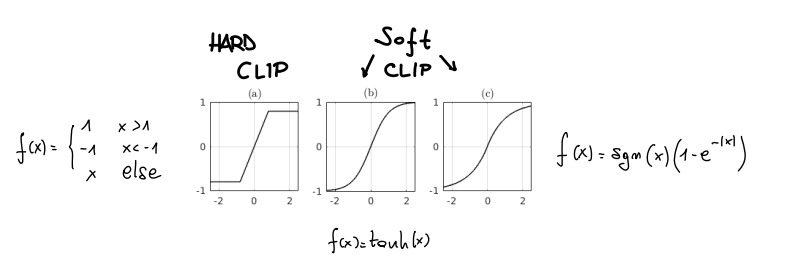
\includegraphics[width=0.7\textwidth]{capitoli/capitolo11/immagini/image1.png}
\end{figure}

\section*{Effetto di Termini Moltiplicativi}

Una moltiplicazione può avere effetti differenti in base alla regione in cui si trova:
\begin{itemize}
    \item Regione quasi lineare $\rightarrow$ semplice moltiplicazione
    \item Regione non lineare $\rightarrow$ effetto molto grande sull’uscita del sistema
\end{itemize}

\section{Effetto di Termini Additivi}

Aggiungendo un termine costante all’ingresso prima della non linearità si ottiene un effetto simile allo spostamento della funzione non lineare.

\section*{Armoniche Pari e Dispari}

\begin{itemize}
    \item Funzioni dispari $\rightarrow$ generano solo armoniche dispari
    \item Funzioni pari $\rightarrow$ generano solo armoniche pari che annullano la fondamentale
    \item Le altre funzioni possono generare qualsiasi tipo di armonica
\end{itemize}

\section{Distorsione}

Funzione non lineare approssimata tramite espansione polinomiale:
\[
y(t) = a_0 + a_1 x + a_2 x^2 + \cdots + a_N x^N
\]

Per valutare l’effetto di distorsione di un segnaloo con un sato polinomio:
\begin{figure}[H]
    \centering
    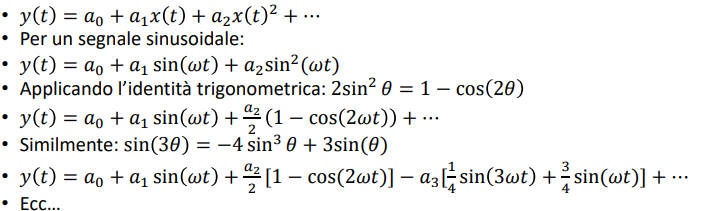
\includegraphics[width=0.7\textwidth]{capitoli/capitolo11/immagini/image2.png}
\end{figure}

\section*{Intermodulazione}

Si consideri un sistema non lineare in cui $f(x_1 + x_2) \neq f(x_1) + f(x_2)$.

\subsection*{1. Espansione non lineare}

\[
y(t) = a_0 + a_1 x(t) + a_2 x(t)^2 + \dots
\]

\subsection*{2. Due segnali sinusoidali in ingresso}

\[
x(t) = \sin(\omega_1 t) + \sin(\omega_2 t)
\]

\[
y(t) = a_0 + a_1[\sin(\omega_1 t) + \sin(\omega_2 t)] + a_2[\sin(\omega_1 t) + \sin(\omega_2 t)]^2 + \dots
\]

\subsection*{3. Sviluppo del termine quadratico}

\[
[\sin(\omega_1 t) + \sin(\omega_2 t)]^2 = \sin^2(\omega_1 t) + \sin^2(\omega_2 t) + 2\sin(\omega_1 t)\sin(\omega_2 t)
\]

Risultano:
\begin{itemize}
    \item \textbf{Componenti armoniche superiori}: $\sin^2(\omega_1 t)$ e $\sin^2(\omega_2 t)$ generano frequenze raddoppiate.
    \item \textbf{Prodotti di intermodulazione}: $\sin(\omega_1 t) \sin(\omega_2 t)$ produce nuove frequenze somma e differenza, come $\omega_1 + \omega_2$ e $\omega_1 - \omega_2$.
\end{itemize}

\subsection*{Conclusioni}

\begin{itemize}
    \item Due segnali sinusoidali in un sistema non lineare generano nuove frequenze.
    \item Frequenze: armoniche superiori e combinazioni $(\omega_1 + \omega_2, \omega_1 - \omega_2)$.
    \item Fenomeno rilevante in elettronica, telecomunicazioni e audio (distorsione indesiderata).
\end{itemize}

\subsection*{Misure}
\begin{itemize}
    \item \textbf{Total Harmonic Distortion (THD)}:
    \[
    THD_F = \frac {\sqrt{V_2^2 + V_3^2 + V_4^2 + \cdots}}{V_1}
    \]
    
    \item \textbf{Signal to Noise Ratio (SNR)}:
    \[
    SNR = \frac{P_{signal}}{P_{noise}}
    \]
    misura la potenza di tutte le parziali inarmoniche.
\end{itemize}

\section{Waveshaping}

\begin{itemize}
    \item utilizza una non linearità applicata a una forma d’onda semplice
    \item semplice e poco costosa
    \item crea spettri complessi
    \item la sintesi FM è un caso particolare di WS
    \item ogni forma d’onda periodica è vista come un seno mandato in una non linearità
    \item spettri che variano nel tempo si possono ottenere moltiplicando l’ingresso per un EG (Envelope Generator)
\end{itemize}

\section*{Look-Up Table (LUT)}

\begin{itemize}
    \item utilizzate in applicazioni di calcolo del suono e della musica
    \item tabella di valori precalcolati (array in memoria)
    \item per ottenere valori intermedi si interpola
    \item basso costo computazionale
    \item la memoria può ridurre le prestazioni (letture frequenti)
    \item le approssimazioni producono errori come distorsione armonica
\end{itemize}

\section*{Aliasing}

\begin{itemize}
    \item funzioni non lineari o clipping generano espansione di banda
    \item nei segnali a tempo discreto si rischia aliasing
    \item si può usare l’oversampling per evitarlo
\end{itemize}

\section*{Wavefolding}

\begin{itemize}
    \item tipo particolare di waveshaping
    \item la funzione non lineare “ribalta” la forma d’onda invece che clipparla o distorcerla
\end{itemize}

\begin{figure}[H]
    \centering
    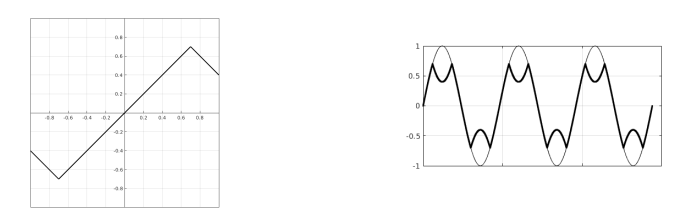
\includegraphics[width=0.7\textwidth]{capitoli/capitolo11/immagini/image3.png}
\end{figure}

\chapter{SINTESI SOTTRATTIVA}
\section*{Sintesi Sottrattiva}

\begin{itemize}
    \item segue l’idea duale
    \item suono ricco spettralmente
    \item elementi fondamentali:
    \begin{itemize}
        \item Oscillatori
        \item Filtri
    \end{itemize}
    \item nata nel mondo analogico
\end{itemize}

Il pilotaggio di segnali è associato a valori controllati di tensioni e correnti.

Nella maggior parte dei sintetizzatori si usa la combinazione VCO (Voltage Controlled Oscillator), VCF (Voltage Controlled Filter), VCA (Voltage Controlled Amplifier) per pilotare gli elementi tempo-varianti.

\begin{figure}[H]
    \centering
    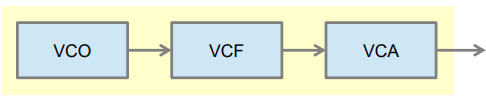
\includegraphics[width=0.7\textwidth]{capitoli/capitolo12/immagini/image1.png}
\end{figure}

\section{Generatori di Rumore}

I rumori possono essere:
\begin{itemize}
    \item Bianchi
    \item Rosa
    \item Marroni
\end{itemize}

\begin{figure}[H]
    \centering
    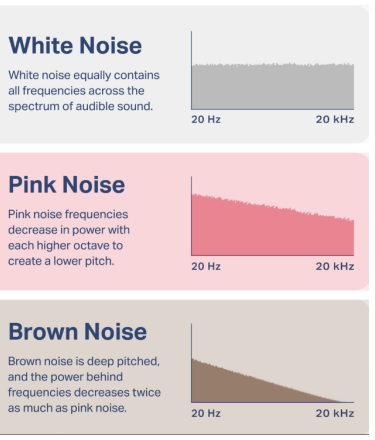
\includegraphics[width=0.7\textwidth]{capitoli/capitolo12/immagini/image2.png}
\end{figure}

Il "colore" del rumore definisce la pendenza di attenuazione dell’energia in funzione della frequenza.

\section{Transistor Ladder Filter (Lowpass)}

\begin{itemize}
    \item basato su una topologia \textit{ladder}
    \item utilizza coppie di transistor differenziali
    \item 4 poli (di solito)
    \item retroazione complessa $\rightarrow$ in tempo discreto si traduce in loop privi di ritardo
    \item può essere altamente non lineare
\end{itemize}
\vspace{8cm}
\section{Sallen-Key Filter}

\begin{itemize}
    \item filtri attivi RC del secondo ordine
    \item non richiedono induttori
    \item realizzati con una cascata di filtri
    \item evitano problemi di sincronizzazione
\end{itemize}

Topologia passa-basso molto comune.

\begin{figure}[H]
    \centering
    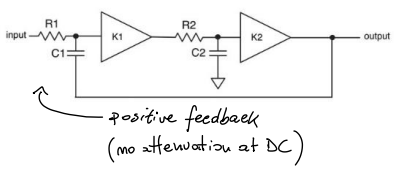
\includegraphics[width=0.7\textwidth]{capitoli/capitolo12/immagini/image3.png}
\end{figure}

\section{State Variable Filter}

\begin{itemize}
    \item composto da due integratori e una retroazione
    \item filtro multimodale
    \item utilizza retroazione negativa
    \item può essere usato come risonatore del secondo ordine perchè il segnale può essere molto basso
\end{itemize}

\begin{figure}[H]
    \centering
    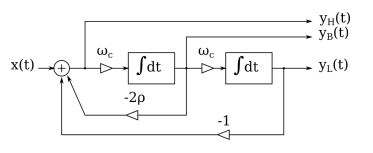
\includegraphics[width=0.7\textwidth]{capitoli/capitolo12/immagini/image4.png}
\end{figure}
\vspace{8cm}
\section{Voltage Controlled Amplifier (VCA)}

\begin{itemize}
    \item controllo dell’ampiezza per aggiungere dinamismo al suono
    \item permette di imitare strumenti acustici
    \item necessita di un generatore di inviluppo (EG / ADSR):
    \begin{itemize}
        \item produce tensione di controllo per impostare l’ampiezza del VCA
        \item i segmenti dell’inviluppo sono:
        \begin{itemize}
            \item \textbf{Attack}
            \item \textbf{Decay}
            \item \textbf{Sustain}
            \item \textbf{Release}
        \end{itemize}
    \end{itemize}
\end{itemize}

\begin{figure}[H]
    \centering
    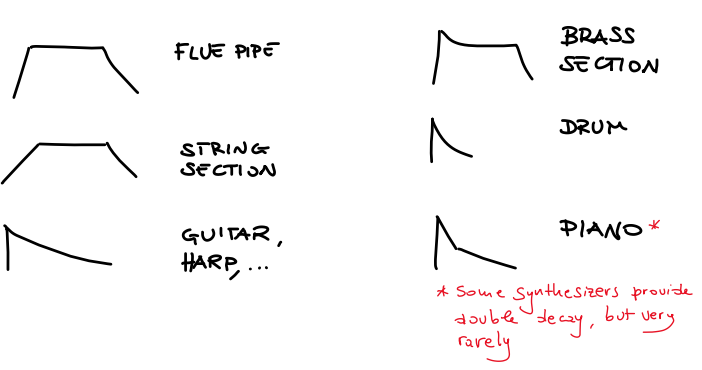
\includegraphics[width=0.7\textwidth]{capitoli/capitolo12/immagini/image5.png}
\end{figure}

\chapter{Sintesi a Campionamento}


\section{Principi di Base}

\begin{itemize}
    \item Il teorema del campionamento garantisce che qualsiasi segnale campionato secondo il teorema di Nyquist può essere perfettamente memorizzato e richiamato per la riproduzione e la conversione D/A.
    \item PCM (Pulse Code Modulation): tecnica usata nei CD audio (16 bit, 44100 Hz).
\end{itemize}
\begin{figure}[H]
    \centering
    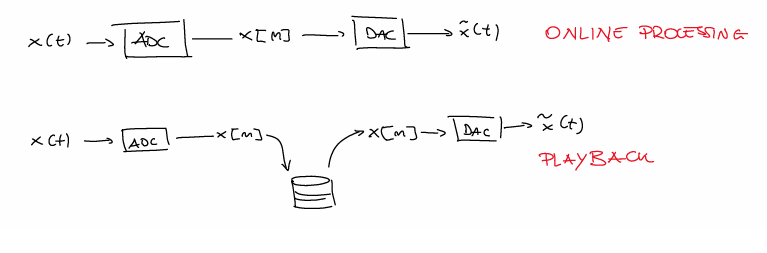
\includegraphics[width=0.7\textwidth]{capitoli/capitolo13/immagini/image1.png}
\end{figure}

\section{Sintesi a Campionamento}

\begin{itemize}
    \item Registrazione, memorizzazione e riproduzione di frammenti sonori.
    \item Adatta per strumenti musicali, voce e suoni complessi.
    \item Non è possibile campionare ogni possibile suono, perciò si rende necessaria una discretizzazione.
\end{itemize}

\section{Esempi: Sintesi a Campionamento}

\subsection{Violino}

\begin{itemize}
    \item \textbf{Pitch}: qualsiasi valore reale nell'intervallo 196--3136 Hz.
    \item \textbf{Forza dell'archetto}: a partire dal valore minimo che produce un tono sostenuto (non un suono stridente).
    \item \textbf{Durata}: da una frazione di secondo a ore.
\end{itemize}

\subsection{Pianoforte}

\begin{itemize}
    \item \textbf{Pitch}: 88 tasti.
    \item \textbf{Velocity}: da pianissimo a fortissimo (approssimativamente da 1 a 50 N).
    \item \textbf{Durata}: da pochi millisecondi a diversi secondi.
\end{itemize}

\noindent
\textit{È impossibile registrare un numero infinito di suoni!}

\section{Discretizzazione dei Dati}

\begin{itemize}
    \item È possibile trovare un modo efficace per discretizzare tutti questi dati.
    \item \textbf{JND (Just Noticeable Difference)} per l'altezza:
    \begin{itemize}
        \item Sotto i 500 Hz: circa 3 Hz per onde sinusoidali, 1 Hz per toni complessi.
        \item Sopra i 1000 Hz: circa 0.6\% per onde sinusoidali (circa 10 cents).
    \end{itemize}
    \item \textbf{Velocity}: piccole variazioni di forza non alterano significativamente il timbro.
    \item \textbf{Durata}: non definita in termini di JND, ma può essere discretizzata in base al contesto.
\end{itemize}

\section{Problemi Aggiuntivi}

\begin{itemize}
    \item \textbf{Pianoforte}: colpire un tasto con il sistema fermo produce un suono diverso rispetto a colpirlo mentre è ancora in vibrazione (ribattuto).
    \item \textbf{Violino}: la posizione dell'archetto sulla corda influisce sul timbro.
\end{itemize}

\noindent
\textit{È davvero impossibile registrare tutti questi suoni! Ma possiamo applicare i principi dell'elaborazione digitale del segnale per modificare pochi suoni registrati e ottenere una grande varietà di risultati.}

\section{Pitch}

\begin{itemize}
    \item Cosa succede se si legge un nastro a velocità diverse?
    \item Possiamo leggere i campioni memorizzati alla velocità desiderata tramite interpolazione.
\end{itemize}
\begin{figure}[H]
    \centering
    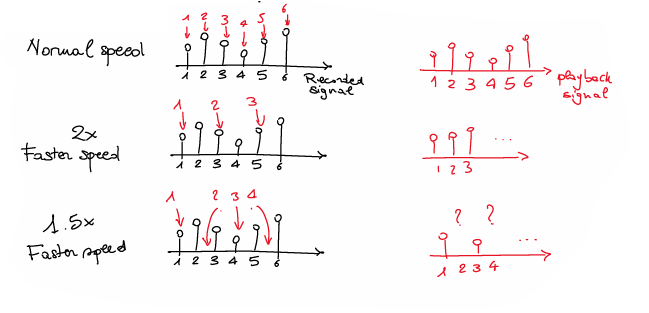
\includegraphics[width=0.7\textwidth]{capitoli/capitolo13/immagini/image2.png}
\end{figure}

\section{Il Problema delle Formanti}

\begin{itemize}
    \item Gli strumenti possono essere approssimati con un modello sorgente-filtro.
    \item Se si modifica l'intonazione variando la velocità di riproduzione, si modificano anche le formanti insieme alle armoniche.
    \item Negli strumenti reali devono cambiare solo le armoniche, non le formanti.
    \item Questo effetto è dovuto alla proprietà di time scaling di Fourier.
    \item Negli strumenti musicali reali siamo però più tolleranti ai cambiamenti di pitch.
\end{itemize}
\begin{figure}[H]
    \centering
    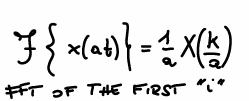
\includegraphics[width=0.3\textwidth]{capitoli/capitolo13/immagini/image3.jpeg}
\end{figure}

\section{Discretizzazione del Pitch}

\begin{itemize}
    \item Un solo tono non è sufficiente; cento sono troppi.
    \item Bisogna trovare un compromesso tra qualità e costi (dipende dall'applicazione e dall’hardware).
    \item Si può usare una discretizzazione approssimativa dell’intervallo di intonazione.
\end{itemize}

\section{Velocity (Intensità)}

\begin{itemize}
    \item È possibile usare un solo campione e modificare l’intensità via guadagno?
    \begin{itemize}
        \item A volte sì, ma raramente.
        \item Spesso non è sufficiente.
    \end{itemize}
    \item La discretizzazione può essere approssimativa:
    \begin{itemize}
        \item Esempio: Key velocity: 0, 30, 80, 127.
    \end{itemize}
    \item Problemi:
    \begin{itemize}
        \item L'aumento della forza può rendere udibili i passaggi di livello se la discretizzazione è troppo grossolana.
        \item Soluzione: somma di due segnali con guadagni complementari.
        \item Problemi della soluzione: costo computazionale doppio, richiede allineamento preciso di fase.
    \end{itemize}
    \item Esempio: Manuale d’uso AKAI S1100 (1990) – spiegazione delle velocity zones.
\end{itemize}

\section{Durata}

\begin{itemize}
    \item Per discretizzare la durata serve conoscere l’evoluzione temporale del segnale.
    \item Esempio: tono dell'organo a canne.
\end{itemize}

\section{Loops}

\begin{itemize}
    \item La scelta dei punti di inizio e fine del loop è molto importante.
\end{itemize}
\begin{figure}[H]
    \centering
    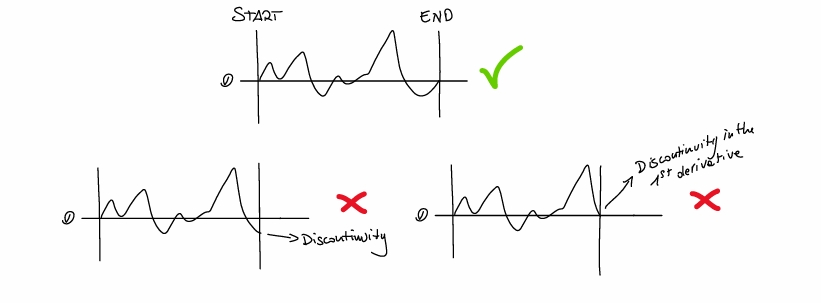
\includegraphics[width=0.7\textwidth]{capitoli/capitolo13/immagini/image4.jpeg}
\end{figure}


\section{Aspetti Tecnici}

\subsection{Costo Computazionale}

\begin{itemize}
    \item Interpolazione tra valori (es. lineare, spline).
    tabread4 = b+frac*\{ cminusb - 0.1666667f * (1.-frac)*[ (d - a - 3.0f * cminusb)*frac + (d + 
2.0f*a – 3.0f*b)]\}
    \item Calcolo di envelope (es. decadimento esponenziale).
    \item Compromesso tra qualità del suono e performance.
\end{itemize}

\subsection{Memoria}

\begin{itemize}
    \item I costi della RAM si sono notevolmente abbassati.
    \item I DSP moderni permettono l’utilizzo di campioni più complessi.
\end{itemize}

\section{Problemi e Limitazioni}

\begin{itemize}
    \item Gli algoritmi che mantengono invariate le formanti sono troppo costosi per l’uso in tempo reale.
    \item Layer dinamici complessi portano a una gestione difficile del timbro.
    \item Mancanza di espressività: tecniche come plettrata, palm mute, bending, ecc., sono difficili da riprodurre.
    \item Soluzioni: round robin (alternanza di campioni), maggiore layering e split, uso del protocollo MPE.
\end{itemize}

\section{Esempi di Sampler Hardware e Software}

\begin{itemize}
    \item AKAI S1100 (1990): 16 bit, 44.1 kHz, 2MB RAM espandibile.
    \item LEM Example (1988): 12 bit, 40.5 kHz.
    \item Elektron Digitakt (2017): 64MB RAM, 1GB storage.
    \item Dream SAM5916B: 16 DSP, 256 voci a 48kHz, decrypting on-the-fly.
\end{itemize}




\chapter{Physical Modeling}

\section{Processi Fisici Generatori di Suono}
Si modellano tutti i processi fisici che portano alla generazione sonora:

\subsection{Circuiti Elettronici Analogici}
\begin{itemize}
  \item Oscillatori
  \item Sorgenti caotiche
  \item Filtri
  \item Circuiti optoelettrici
\end{itemize}

\subsection{Sistemi Acustici}
\begin{itemize}
  \item Tubi (1D)
  \item Corde (1D)
  \item Piastre (2D)
  \item Stanze (3D)
\end{itemize}

\section{Tipi di Processi Fisici}
I processi fisici di interesse sono lineari, non lineari o addirittura caotici:

\begin{itemize}
  \item Propagazione delle onde (solitamente isotrope e lineari) e generazione di onde stazionarie in un mezzo o in un risonatore
  \item Eccitazione di un risonatore
  \item Interazione rigida/elastica non lineare tra corpi
\end{itemize}

\section{Modellazione a Tempo Continuo e Discreto}
\begin{itemize}
  \item Generalmente un modello a tempo continuo è derivato in termini di equazioni differenziali
  \item Questi possono essere estremamente complessi per essere risolti in tempo reale, si possono applicare delle approssimazioni
  \item Un esempio di approssimazione è la teoria modale
  \item Viene quindi derivato un modello a tempo discreto per eseguire il calcolo su un computer
\end{itemize}

\section{Domini Fisici e Variabili}
Tutti i domini fisici di interesse sono descritti da quantità misurabili che di solito si presentano in coppie di variabili:

\begin{itemize}
  \item Meccanica: Forza + Velocità
  \item Acustica: Pressione + Velocità del volume
  \item Elettrico: Tensione + Corrente
  \item In generale: variabile "trasversale" (o "potenziale") + variabile "passante" (o "cinetica")
\end{itemize}

La tensione è il potenziale "attraverso" due terminali e la corrente è il flusso di elettroni "attraverso" una sezione.

\section{Paradigmi di Modellazione}
\subsection{Paradigma 1: K-variables}
K-variables, o Kirchhoff variables: utilizza la coppia «across» e «through» (trasversale e passante)

\begin{itemize}
  \item Questo fornisce una soluzione diretta del sistema
  \item Può essere utilizzato per scomporre il sistema nei suoi modi naturali
\end{itemize}

\subsection{Paradigma 2: W-variables}
Astrazione: utilizzare il concetto astratto di "onde".

\begin{itemize}
  \item Variabili W, o variabili d'onda: onde incidenti e riflesse
  \item Le onde sono astrazioni che si sommano per comporre le grandezze osservabili K
\end{itemize}
\section{1D Wave Eq. and Solutions}

\subsection{Digital Waveguides}

\begin{itemize}
  \item I Digital Waveguides seguono l’approccio W-domain, ma non devono essere confusi con gli Wave-Digital Filters.
  \item Forniscono un modo molto economico per modellare la propagazione delle onde in condizioni ideali per problemi 1D.
  \item Per problemi 2D e 3D possono essere impiegati, ma il costo computazionale non è più conveniente rispetto ad altri approcci.
\end{itemize}

\section{Caso 1D}

La propagazione di una grandezza \( y \) in un mezzo, ad esempio la propagazione di un'onda di velocità in una corda rigida ideale, può essere modellata come:

\[
\frac{d^2 y}{dt^2} = c^2 \frac{d^2 y}{dx^2}
\]

dove \( c \) è la velocità di propagazione.

\subsection{Soluzione a questa PDE}

La prima soluzione a questa equazione alle derivate parziali (PDE) fu data da D'Alembert nel 1747:

\[
y(x, t) = y^+ \left( t - \frac{x}{c} \right) + y^- \left( t + \frac{x}{c} \right)
\]

Ciò significa che il valore della variabile al tempo \( t \) e nella posizione \( x \) può essere calcolato dalla sovrapposizione di due onde viaggianti: un'onda progressiva \( y^+ \) e un'onda regressiva \( y^- \) di forma arbitraria.

\section{Somma di Onde Progressive e Regressive}

La soluzione al caso 1D è rappresentata dalla somma di onde progressive e regressive.

\section{Discretizzazione della Soluzione di D'Alembert}

La formulazione dei Digital Waveguides (DWG) è ottenuta mediante discretizzazione della soluzione di D'Alembert. La stringa è discretizzata a intervalli spaziali regolari:

\[
x_m = m \Delta x, \quad m \in \{0, \dots, M\}
\]

Il valore di ogni punto viene calcolato a intervalli di tempo regolari:

\[
t_n = n \Delta t, \quad n \in \{0, \dots, N\}
\]

L'equazione d'onda può quindi essere riscritta come:
\begin{figure}[H]
    \centering
    
\includegraphics[width=0.7\textwidth]{capitoli/capitolo14/immagini/image1.jpeg}
\end{figure}

\[
\text{(equazione d'onda discretizzata)}
\]

\section{Condizione di Stabilità e Alias Spaziale}

La selezione dell'intervallo di campionamento spaziale è fondamentale per la stabilità e per evitare l'aliasing spaziale. La condizione di stabilità di Von Neumann impone che:

\[
\frac{c \Delta t}{\Delta x} \leq 1
\]

\section{Formulazione DWG e Diagramma di Flusso}

La formulazione dei Digital Waveguides corrisponde al seguente diagramma di flusso:
\begin{figure}[H]
    \centering
    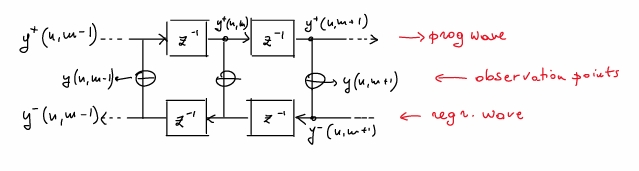
\includegraphics[width=0.7\textwidth]{capitoli/capitolo14/immagini/image2.jpeg}
\end{figure}

\section{Terminazioni "Rigide"}

Le condizioni al contorno sono fondamentali per definire il problema. Un caso tipico è la terminazione rigida: ad esempio, la corda non può muoversi ai suoi estremi. Questo è imposto dall'avere:

\begin{itemize}
  \item Le condizioni di terminazione rigida specificano che la velocità della corda alle estremità sia zero.
\end{itemize}

\section{Aggregazione}

Se possiamo accettare di non calcolare l'uscita in tutte le posizioni, possiamo semplificare il modello utilizzando un approccio di aggregazione:

\begin{itemize}
  \item Si riduce la complessità computazionale, trascurando alcune informazioni spaziali in favore di un'efficienza maggiore.
\end{itemize}

\begin{figure}[H]
    \centering
    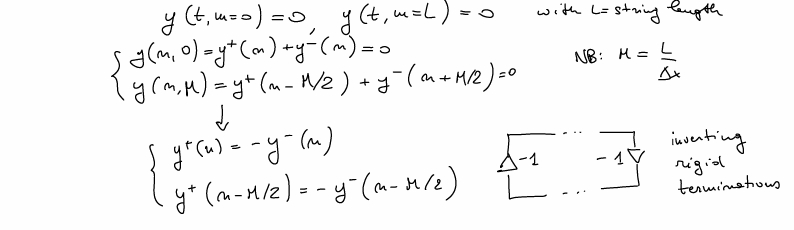
\includegraphics[width=0.7\textwidth]{capitoli/capitolo14/immagini/image3.jpeg}
\end{figure}

\section{Perdite}

In realtà, il mezzo non è privo di perdite e può presentare attriti. La soluzione è ora espressa come onde viaggianti a decadimento esponenziale:

\begin{itemize}
  \item La perdita di energia è modellata come un termine che rappresenta il decadimento esponenziale dell'onda mentre si propaga.
\end{itemize}

\begin{figure}[H]
    \centering
    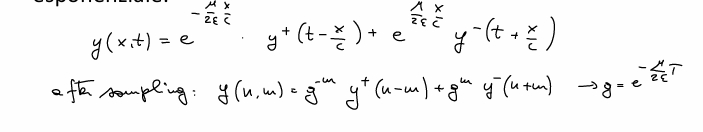
\includegraphics[width=0.7\textwidth]{capitoli/capitolo14/immagini/image4.jpeg}
\end{figure}

\section{Perdite Dipendenti dalla Frequenza}

Il termine di attrito è solo un'approssimazione. È possibile introdurre termini di perdita aggiuntivi per approssimare un comportamento dipendente dalla frequenza. La soluzione si generalizza ora a:

\begin{itemize}
  \item Le perdite dipendenti dalla frequenza sono modellate come un filtro che modula l'attenuazione in funzione della frequenza.
\end{itemize}

\section{Aggregazione di Perdite Dipendenti dalla Frequenza}

I termini dipendenti dalla frequenza possono essere consolidati come un filtro. Questo approccio consente di modellare in modo più preciso le perdite, specialmente in sistemi con comportamento non lineare o con forti variazioni di impedenza.

\begin{itemize}
  \item Utilizzare un filtro permette di simulare in modo efficiente i cambiamenti nelle perdite a seconda della frequenza, migliorando la realismo del modello.
\end{itemize}


\section{Dispersione}

La rigidità di una corda vibrante introduce una forza di ripristino proporzionale alla quarta derivata dello spostamento della corda.

\section{Effetto di Dispersione}

L'effetto di primo ordine della rigidità è l'aumento della velocità di propagazione delle onde con la frequenza:

\[
\omega = \omega_0 \left( 1 + \frac{2K}{c_0^2} \right)
\]

Pertanto, le onde che viaggiano si "disperdono" mentre attraversano la corda. Le componenti ad alta frequenza si propagano più velocemente.

\section{Decomposizione Modale}

L'effetto di dispersione può essere studiato utilizzando una decomposizione modale.

\section{Ritardi Dipendenti dalla Frequenza}

La dispersione richiede ritardi dipendenti dalla frequenza. Se possiamo aggregare, un'opzione conveniente è l'utilizzo di filtri Allpass.

\section{Fractional Delays}

Come intonare una Digital Waveguide (DWG)?

\begin{itemize}
    \item Finché il numero di tappi \( N \in \mathbb{N} \), il numero delle frequenze ottenibili è un insieme discreto.
    \item Per dividere un delay unitario, dobbiamo ricorrere a dei delay frazionari.
\end{itemize}

\section{Discrete-Time Arbitrary Delay}

\begin{figure}[H]
    \centering
    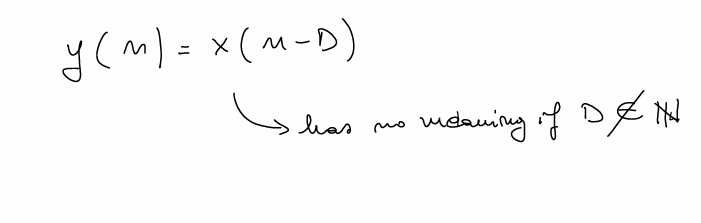
\includegraphics[width=0.7\textwidth]{capitoli/capitolo14/immagini/image5.jpeg}
\end{figure}

L'interpolazione del valore tra due intervalli di campionamento successivi è equivalente alla ricostruzione del segnale a tempo continuo dai valori discreti secondo il campionamento Shannon-Nyquist. Pertanto, l'interpolatore ideale è esattamente il filtro di ricostruzione!

\[
\text{Il fractional-delay ideale è quindi un filtro di ricostruzione.}
\]

%dove mi sono fermato
\section{Discrete-Time Arbitrary Delay}

Quando \( 0 < d < 1 \), l'IR risultante è infinito, non causale e non stabile BIBO (non assolutamente sommabile). Possiamo solo approssimare il ritardo frazionario ideale.

\subsection{Dominio della Frequenza}
Guardando al dominio della frequenza:

\begin{itemize}
    \item Tuttavia, nessun filtro con coefficienti reali può essere complesso a Nyquist.
    \item Questo significa che l'errore di approssimazione sarà almeno \( \sin\left( \frac{\pi D}{2} \right) \), il che è noto come il vincolo di Tarczynski.
\end{itemize}

\section{Fractional Delay Ideale (Tempo Continuo)}

Il ritardo continuo (frazionario) nel tempo e nella frequenza è rappresentato come un filtro ideale di fase lineare all-pass.

\begin{figure}[H]
    \centering
    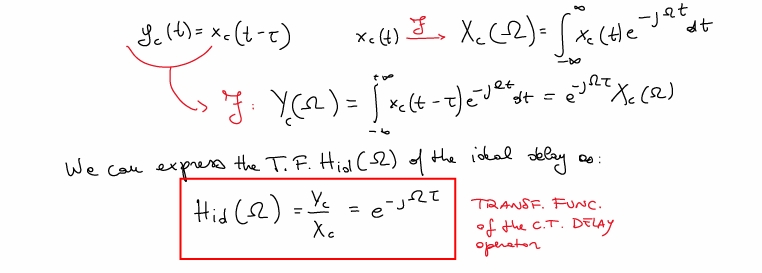
\includegraphics[width=0.7\textwidth]{capitoli/capitolo14/immagini/image6.jpeg}
\end{figure}


\subsection{Caratteristiche in Frequenza}

Il fractional delay ideale è un filtro all-pass di fase lineare.

\begin{figure}[H]
    \centering
    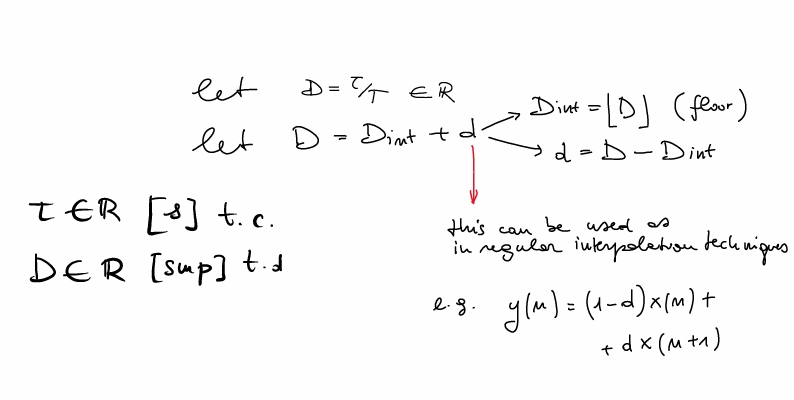
\includegraphics[width=0.7\textwidth]{capitoli/capitolo14/immagini/image7.jpeg}
\end{figure}


\section{Progettazione del Filtro Interpolatore}

Il ritardo frazionario può essere approssimato da un filtro FIR o da un filtro IIR.

\subsection{Metodi di Progettazione FIR}

\begin{itemize}
    \item Troncamento dell'IR, progettazione ai minimi quadrati, approssimazione polinomiale, ecc.
    \item Vantaggi: i coefficienti possono essere modificati senza problemi di stabilità.
\end{itemize}

\subsection{Metodi di Progettazione IIR}

\begin{itemize}
    \item Basato su design all-pass.
    \item Vantaggi: ritardi più elevati con costi di calcolo inferiori.
    \item FLIPPED CLASSROOM: Thiran Allpass.
\end{itemize}

\section{Strumenti ad Ancia}

\begin{itemize}
    \item Se il bore è cilindrico, come nel caso del clarinetto, può essere modellato semplicemente utilizzando una linea di ritardo bidirezionale.
    \item Se il bore è conico, come nel caso del sassofono, può essere modellato come una linea di ritardo bidirezionale, ma l'interfacciamento con esso è più complesso, soprattutto in corrispondenza dell'imboccatura.
    \item Il filtro d'uscita è un filtro peak che definisce la campana di risonanza.
    \item Il filtro di riflessione modella il comportamento in frequenza del bore.
    \item Il modello dell'ancia è essenzialmente una non linearità molto "orizzontale".
\end{itemize}

\section{Strumenti ad Arco}

\begin{itemize}
    \item La coppia di linee di ritardo di destra trasporta i campioni delle onde di velocità di sinistra e di destra (Bridge to Bow delay).
    \item La velocità della corda in qualsiasi punto si ottiene sommando un campione di velocità in direzione sinistra al campione di velocità in direzione destra immediatamente opposto nell'altra linea di ritardo.
    \item Il filtro di riflessione a destra implementa le perdite al ponte, all'archetto, al capotasto o alle terminazioni delle dita (quando sono ferme), e l'attenuazione/dispersione di andata e ritorno dalla corda.
    \item Con un ottimo grado di approssimazione, il nut riflette le onde di velocità in entrata (con un'inversione di segno) a tutte le lunghezze d'onda.
    \item L'interpolazione delle linee di ritardo può essere utilizzata per fornire un cambiamento continuo della posizione dell'arco.
\end{itemize}

\section{Strumenti ad Aria (Flue)}

\begin{itemize}
    \item La generazione sonora è composta dal rumore del "soffio" che entra nella sezione risonante.
    \item La generazione armonica è "arricchita" dalla non linearità \( x - x^3 \) che modella la parte di energia che ritorna dalla canna al momento dell’insorgere della pressione.
    \item Il decadimento in frequenza è dato dal filtro LP nell'anello della "flue bore DL".
    \item La combinazione dell'effetto dei due anelli intona la nota. Tipicamente la DL bore corrisponde alla lunghezza d'onda della nota, mentre la DL dell'imboccatura è metà della DL di bore.
    \item Il modello può essere reso più stabile.
\end{itemize}

\chapter{Filtri per mastering}

\section{Introduzione}

\begin{itemize}
    \item Idealmente, la risposta in frequenza netta di un sistema dovrebbe essere uniforme per tutte le frequenze: da qui deriva il termine ``equalizzazione''.
    
    \item Il termine ``equalizzazione'' è stato utilizzato per indicare qualsiasi procedura che comporti l'alterazione o la regolazione della risposta in frequenza dell’ampiezza di un segnale.
    
    \item Il concetto di filtraggio delle frequenze audio è noto almeno fin dagli anni '70 del XIX secolo, ed è stato applicato nei primi progetti di telegrafi armonici.
    
    \item Le linee telefoniche venivano equalizzate nei ripetitori utilizzando filtri d'onda per annullare le risonanze causate da disadattamenti di impedenza o dall'attenuazione delle alte frequenze nei cavi lunghi.
    
    \item Il termine ``filtro'' può assumere numerosi significati. Un filtro seleziona le componenti del segnale in base alle frequenze che si desidera rifiutare, mantenere o enfatizzare.
    
    \item I filtri sono comunemente descritti nel dominio della frequenza, ma hanno anche effetti significativi nel dominio del tempo.
    
    \item Oltre alla loro funzione di modulazione della frequenza, i filtri possono essere analizzati nel dominio temporale, dando origine a una famiglia di effetti audio basati sul ritardo, come quelli che si possono sperimentare negli spazi acustici.
\end{itemize}

\section{Filtri base}

\begin{itemize}
    \item \textbf{Filtri passa-basso (LP)}: selezionano le basse frequenze fino alla frequenza di taglio $f_c$ e attenuano le frequenze superiori a $f_c$. Inoltre, una risonanza può amplificare le frequenze intorno a $f_c$.

    \item \textbf{Filtri passa-alto (HP)}: selezionano le frequenze superiori a $f_c$ e attenuano quelle inferiori, con la possibilità di una risonanza attorno a $f_c$.

    \item \textbf{Filtri passa-banda (BP)}: selezionano le frequenze comprese tra una frequenza di taglio inferiore $f_{cl}$ e una superiore $f_{ch}$.

    \item \textbf{Filtri bandreject (BR)}: attenuano le frequenze comprese tra $f_{cl}$ e $f_{ch}$, lasciando passare quelle al di fuori di questo intervallo.

    \item \textbf{Filtri all-pass}: permettono il passaggio di tutte le frequenze, ma modificano la fase del segnale in ingresso.
\end{itemize}


\begin{itemize}
    \item Il filtro passa-basso con risonanza è molto utilizzato nella computer music per simulare una struttura acustica risonante.

    \item Il filtro passa-alto è utile per rimuovere frequenze molto basse indesiderate.

    \item Il passa-banda può produrre effetti come l'imitazione di una linea telefonica o di una sordina applicata a uno strumento acustico.

    \item Il bandreject può dividere lo spettro udibile in due bande che risultano percepite come non correlate.
\end{itemize}

\section{Filtri canonici}

\begin{itemize}
    \item Esistono diversi modi per implementare un filtro. Il più semplice è il filtro canonico, spesso utilizzato per realizzare filtri del secondo ordine mediante equazioni alle differenze.
    
    \begin{figure}[H]
        \centering
        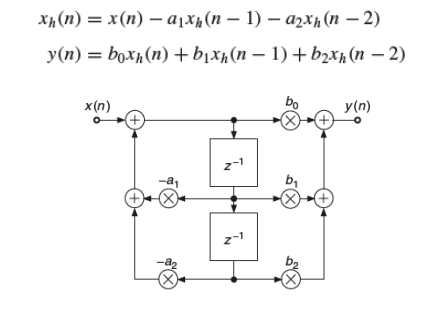
\includegraphics[width=0.7\textwidth]{capitoli/capitolo15/immagini/image1.png}
    \end{figure}
    

    \item A seconda dei coefficienti $a$ e $b$, si possono ottenere diversi comportamenti del filtro. Da tali coefficienti si ottiene la funzione di trasferimento del sistema.
    
    \begin{figure}[H]
        \centering
        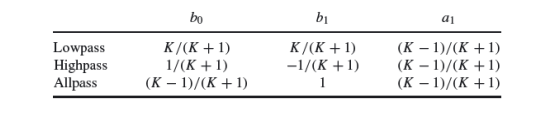
\includegraphics[width=0.7\textwidth]{capitoli/capitolo15/immagini/image2.png}
    \end{figure}

    \item Impostando $a_2 = b_2 = 0$, il filtro si riduce a un filtro del secondo ordine. Questo può essere utilizzato per implementare un filtro passa-tutto, passa-basso o passa-alto, con i coefficienti forniti in apposite tabelle. Il parametro $K$ dipende dalla frequenza di taglio.
    
    \item Nel filtro passa-tutto, il coefficiente $K$ controlla anche la frequenza $f_c$ alla quale si raggiunge uno sfasamento di $-90^\circ$.
\end{itemize}


\begin{itemize}
    \item Per i filtri del secondo ordine, oltre alla frequenza di taglio (o frequenza centrale), è necessario specificare anche il fattore $Q$, che assume significati diversi a seconda del tipo di filtro:
    
    \begin{itemize}
        \item Nei filtri passa-basso e passa-alto, $Q$ controlla l'altezza della risonanza. Per $Q = \frac{1}{\sqrt{2}}$, il filtro risulta massimamente piatto fino alla frequenza di taglio. Per valori inferiori di $Q$, si ha una maggiore attenuazione in banda passante; per valori superiori, si osserva un'amplificazione attorno a $f_c$.
        
        \item Nei filtri passa-banda e bandreject, $Q$ è legato alla larghezza di banda $f_b$ secondo la relazione $Q = \frac{f_c}{f_b}$, ovvero è l'inverso della larghezza di banda relativa $\frac{f_b}{f_c}$.
        
        \item Nel filtro passa-tutto, $Q$ controlla anch'esso la larghezza di banda, che in questo caso è definita dai punti in cui si raggiungono $\pm 90^\circ$ di sfasamento, rispetto ai $-180^\circ$ raggiunti in corrispondenza di $f_c$.
    \end{itemize}
    
    \item Sebbene i filtri canonici siano relativamente semplici dal punto di vista concettuale, il calcolo dei loro coefficienti a partire da parametri come la frequenza di taglio e la larghezza di banda può risultare complesso.
\end{itemize}

\begin{figure}[H]
    \centering
    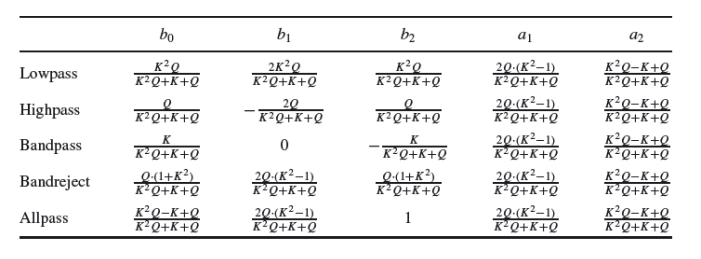
\includegraphics[width=0.7\textwidth]{capitoli/capitolo15/immagini/image3.png}
\end{figure}

\section{State Variable Filter}

\begin{itemize}
    \item Un'interessante alternativa alla struttura del filtro canonico è il \textit{filtro a variabili di stato}, che combina filtri passa-basso, passa-banda e passa-alto del secondo ordine, mantenendo la stessa frequenza di taglio $f_c$ e lo stesso fattore di qualità $Q$.

    \begin{figure}[H]
        \centering
        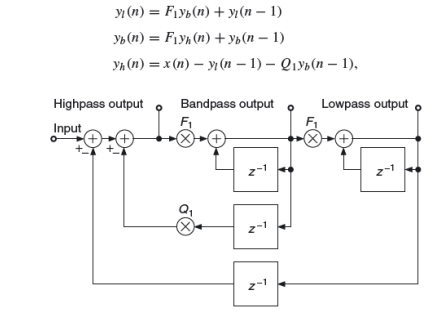
\includegraphics[width=0.7\textwidth]{capitoli/capitolo15/immagini/image4.png}
    \end{figure}

    \item I coefficienti di sintonizzazione $F_1$ e $Q_1$ sono correlati ai parametri $f_c$ e $Q$.

    \item Si può dimostrare che le funzioni di trasferimento per i tre tipi di filtro (passa-basso, passa-banda e passa-alto) dipendono dai parametri $r = F_1$ e $q = 1 - F_1 Q_1$.
\end{itemize}
\begin{figure}[H]
    \centering
    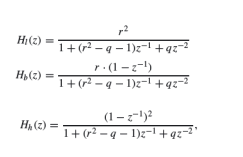
\includegraphics[width=0.3\textwidth]{capitoli/capitolo15/immagini/image5.png}
\end{figure}

\begin{itemize}
    \item Questa struttura è particolarmente efficace non solo nel processo di filtraggio, ma soprattutto per la semplicità delle relazioni tra i parametri di controllo e i coefficienti di sintonizzazione.

    \item È necessario considerare la stabilità del filtro: a frequenze di taglio elevate e per valori di $Q$ molto piccoli, il filtro può diventare instabile.

    \item Per garantire il funzionamento stabile del filtro a variabili di stato, è utile rispettare il limite di utilizzabilità dato dalla condizione:
    
    \[
    F_1 < 2 - Q_1
    \]

    \item Le proprietà di questo filtro sono state sfruttate in applicazioni creative, ad esempio per produrre glissandi infiniti a partire da suoni naturali, oppure per permettere transizioni fluide tra configurazioni estreme.
\end{itemize}

\section{Filtri all-pass}

\begin{itemize}
    \item Un filtro all-pass ha un comportamento piatto come risposta in frequenza del modulo.

    \item Può essere descritto come segue:

    \[
    H(s) = \frac{b(s)}{a(s)}
    \]

    dove $b(s)$ e $a(s)$ sono polinomi in $s$.

    \item Il filtro all-pass corrisponde a uno schema a blocchi del tipo:

    \begin{figure}[H]
        \centering
        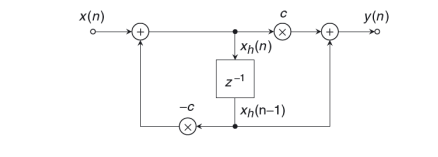
\includegraphics[width=0.7\textwidth]{capitoli/capitolo15/immagini/image6.png}
    \end{figure}
\end{itemize}


\begin{itemize}
    \item Dai filtri all-pass, combinando opportunamente gli elementi, è possibile derivare altre tipologie di filtro.
    
    \item La funzione di trasferimento di un filtro all-pass del secondo ordine è data da:

    \begin{figure}[H]
        \centering
        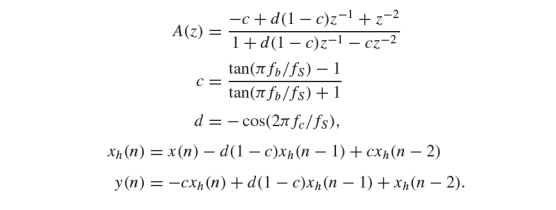
\includegraphics[width=0.7\textwidth]{capitoli/capitolo15/immagini/image7.png}
    \end{figure}

    dove $\zeta$ è il fattore di smorzamento e $\omega_n$ è la frequenza centrale.

    \item Il parametro $d$ regola la frequenza centrale e il parametro $c$ la larghezza di banda.
\end{itemize}

\bigskip

\begin{itemize}
    \item Gli all-pass del secondo ordine possono essere utilizzati per implementare in maniera efficace filtri passa-banda (BP) e bandreject (BR).
\end{itemize}

\section{FIR filters}

\begin{itemize}
    \item I filtri digitali che abbiamo visto in precedenza hanno una risposta all'impulso infinita.
    
    \item Al contrario, la risposta all’impulso per i filtri FIR è di durata finita.
    
    \item Questi filtri consentono di costruire tipi di filtro sofisticati, dove è necessaria una forte attenuazione delle frequenze indesiderate o la scomposizione del segnale in diverse bande di frequenza.
\end{itemize}

\section{FIR Comb filters(DOMANDA CERTA ALL'ESAME)}

\begin{itemize}
    \item Il segnale di ingresso viene ritardato di un determinato tempo. L'effetto sarà udibile solo quando il segnale elaborato viene combinato (aggiunto) al segnale di ingresso, che funge da riferimento. Questo effetto ha due parametri di regolazione:
    
    \begin{itemize}
        \item L'entità del ritardo $\tau$.
        
        \item L'ampiezza relativa del segnale ritardato rispetto a quella del segnale di riferimento.
    \end{itemize}
\end{itemize}

\begin{figure}[H]
    \centering
    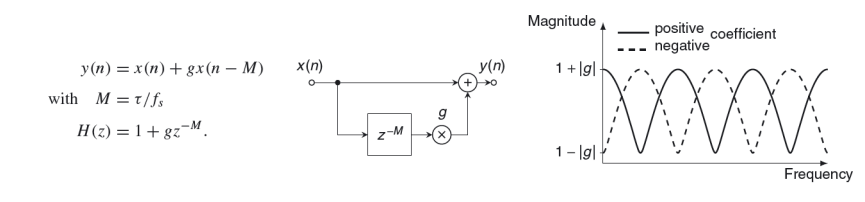
\includegraphics[width=0.7\textwidth]{capitoli/capitolo15/immagini/image8.png}
\end{figure}

\section{IIR Comb filters}

\begin{itemize}
    \item Imitando le infinite riflessioni alle due estremità di un cilindro, il filtro comb IIR produce una serie infinita di risposte $y(n)$ a un ingresso $x(n)$.
    
    \item Il segnale d'ingresso circola in una linea di ritardo che viene reintrodotta in ingresso.
\end{itemize}

\begin{figure}[H]
    \centering
    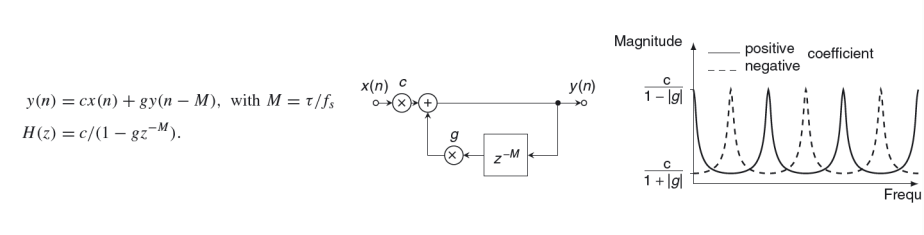
\includegraphics[width=0.7\textwidth]{capitoli/capitolo15/immagini/image9.png}
\end{figure}

\section{Universal Comb filters}

\begin{itemize}
    \item La combinazione dei filtri comb FIR e IIR conduce al filtro comb universale.
    
    \item Questa struttura di filtro si trasforma in una struttura all-pass nel caso speciale di $-BL = FB$, $FF = 1$, dove il ritardo a un campione $z^{-1}$ è sostituito dal ritardo a $M$ campioni $z^{-M}$.
\end{itemize}

\section{Shelving filters (I order)}

\begin{itemize}
    \item In maniera simile ai filtri LP/HP che possono essere costruiti partendo da degli all-pass, si possono ottenere filtri shelving del primo ordine partendo da all-pass del primo ordine con funzione di trasferimento $A(z)$.
\end{itemize}

\begin{itemize}
    \item I parametri di Cutoff boost ($C_b$) e Cutoff cut ($C_c$) variano a seconda del tipo di shelving filter desiderato:
    \begin{figure}[H]
        \centering
        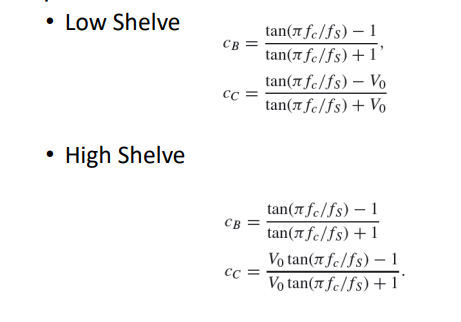
\includegraphics[width=0.7\textwidth]{capitoli/capitolo15/immagini/image10.png}
    \end{figure}
\end{itemize}
\vspace{5cm}
\section{Shelving filters (II order)}

\begin{itemize}
    \item Per diverse applicazioni, la pendenza del filtro shelving viene ulteriormente aumentata da funzioni di trasferimento di secondo ordine o superiore.
    
    \item Esistono diversi approcci per progettare filtri shelving di ordine superiore con un calcolo relativamente semplice dei coefficienti, al costo di strutture di filtro leggermente più complicate.
\end{itemize}
\begin{figure}[H]
    \centering
    \includegraphics[width=0.7\textwidth]{capitoli/capitolo15/immagini/image11.png}
\end{figure}

\section{Peak filters}

\begin{itemize}
    \item In maniera analoga, un filtro peak del secondo ordine può essere derivato sfruttando un all-pass del secondo ordine.
\end{itemize}
\begin{figure}[H]
    \centering
    \includegraphics[width=0.7\textwidth]{capitoli/capitolo15/immagini/image12.png}
\end{figure}
\vspace{8cm}
\section{EQ}

\begin{itemize}
    \item A differenza dei filtri passa-basso/alto e passa/elimina-banda, che attenuano lo spettro audio al di sopra o al di sotto di una frequenza di taglio, gli equalizzatori modellano lo spettro audio modificando alcune bande di frequenza mentre altre rimangono inalterate.
    
    \item In genere, gli equalizzatori sono costruiti con un collegamento in serie di filtri shelving e di picco del primo e del secondo ordine, controllati in modo indipendente.
\end{itemize}

\section{GEQ (equalizzatori grafici)}

\begin{itemize}
    \item L'equalizzatore grafico è uno strumento che consente di regolare in modo indipendente il guadagno di più regioni di frequenza in un segnale audio.
    
    \item I comuni equalizzatori grafici possono fornire fino a circa 30 controlli per la manipolazione della risposta in frequenza di ciascun canale audio.
    
    \item Strutturalmente, un equalizzatore grafico è un insieme di filtri, ciascuno con una frequenza centrale e una larghezza di banda fisse. L'unico controllo da parte dell'utente è il guadagno di comando, ovvero la quantità di incremento o di taglio in ciascuna banda di frequenza.
\end{itemize}

\bigskip

\begin{itemize}
    \item Il guadagno di ciascuna banda di frequenza può essere solitamente regolato entro un intervallo di 12 dB, corrispondente a circa $0.25 < G < 4$ per ciascun filtro.
    
    \item Il termine \textit{grafico} si riferisce al fatto che la posizione delle manopole dei cursori può essere intesa come un grafico della risposta in magnitudine dell'equalizzatore.
    
    \item Un equalizzatore grafico può essere implementato utilizzando una cascata di filtri equalizzatori o un banco parallelo di filtri passa-banda.
    
    \item In un'implementazione a cascata, ogni filtro determina la risposta intorno alla frequenza centrale in base al proprio guadagno (peak filters, guadagno 1 fuori banda).
    
    \item In un'implementazione parallela, ogni filtro passa-banda produce alla sua frequenza centrale un guadagno determinato dal guadagno del suo comando (BP filters, guadagno –inf fuori banda).
\end{itemize}

\chapter{Effetti basati su DL}

\section{Lista di effetti basati su Delay Line}
\begin{itemize}
    \item Digital Delay
    \item Reverb
    \item Chorus
    \item Flanger
    \item Vibrato
\end{itemize}

\section{Delay Line}
\textbf{• Con il termine Delay Line si intende un buffer di memoria lungo Nsamples nel quale viene scritto un dato e successivamente viene letto}
\textbf{• Time = distanza tra i puntatori di scrittura e lettura}

\section{Vibrato}
\textbf{Il dato viene letto a diverse velocità così da cambiarne il pitch}

\section{Slapback/Echo/Delay}
\begin{itemize}
    \item \textbf{Slapback}(o doubling): 10 < M < 25 ms
    \item \textbf{Echo}: M > 50 ms
    \item g setta il dry/wet
\end{itemize}

\begin{itemize}
    \item \textbf{Delay}(simula multiple riflessioni)
    \item g setta il dry/wet
\end{itemize}

\section{Flanger/Chorus}
\begin{itemize}
    \item \textbf{Flanger}: M < 15 ms, variabile periodicamente (LFO)
    \item \textbf{Chorus}: generato da copie del segnale a pitch leggermente modificati: si usa il delay che genera più vibrato, sommati al segnale diretto
    \item M1, M2 10-25 ms, diversi tra loro
\end{itemize}

\section{Phaser}
\begin{itemize}
    \item L'orecchio umano non è molto sensibile alle differenze di fase, ma questo crea interferenze udibili quando viene mixato con il segnale dry (non processato), creando dei notch.
    \item Il numero di filtri all-pass (solitamente chiamati stadi) varia a seconda dei modelli; alcuni phaser analogici offrono 4, 6, 8 o 12 stadi.
\end{itemize}

\section*{Riverbero}

\begin{itemize}
    \item La riverberazione naturale è una condizione tipica degli ambienti spazialmente delimitati (stanze, auditorium, chiese, teatri, ecc).
    
    \item Ogni ambiente ha una propria e caratteristica riverberazione (si pensi al tipico riverbero di una chiesa o di un cinema).
    
    \item In natura, gli ambienti privi di riverbero sono una condizione molto difficile da avere.
    
    \item Esistono apposite camere dette anecoiche, le quali sono studiate per eliminare le riverberazioni ambientali.
\end{itemize}

\begin{itemize}
    \item In rosso: 
    \begin{itemize}
        \item Il path diretto dalla sorgente all’ascoltatore.
    \end{itemize}
    
    \item In blu:
    \begin{itemize}
        \item Le riflessioni ambientali (riverbero).
    \end{itemize}
    
    \item Esistono diverse tipologie di riflessioni a seconda di quanti «rimbalzi» ci sono tra sorgente e ascoltatore.
\end{itemize}

\section{Room Impulse Response (RIR)}
\begin{itemize}
    \item La caratterizzazione di un ambiente è un tema molto importante nel Sound Design.
    
    \item Ogni ambiente ha il suo tipico riverbero ambientale.
    
    \item Modellare correttamente un ambiente, in termini di riverbero, molto spesso è fondamentale al fine di avere un sound design musicale ed efficace.
    
    \item Possiamo distinguere differenti «componenti» di un segnale riverberato:
    \begin{itemize}
        \item Suono diretto (Dry)
        \item Early Reflections
        \item Late riverberation
        \item Decay Rate
        \item Predelay (T0)
    \end{itemize}
\end{itemize}

\section{Reverberation Time}

\begin{itemize}
    \item Il Reverberation Time misura il cosiddetto $T_{60}$, cioè il tempo dopo il quale il segnale di riverbero è attenuato di 60 dB rispetto al suo livello di partenza.
    
    \item Il $T_{60}$, in natura, è funzione di differenti fattori:
    \begin{itemize}
        \item Dimensioni $W \times L \times H$ dell’ambiente
        \item Materiali costruttivi delle pareti (riflettenti e non)
        \item Elementi acustici ambientali
    \end{itemize}
\end{itemize}

\section{Effetto del pre-delay}
\begin{itemize}
    \item Il pre-delay tra il segnale diretto e la sua replica ha i seguenti effetti dipendenti dal tempo:
    \begin{itemize}
        \item $< 50$ ms: Haas effect, o doubling
        \item $50 < \text{delay} < 100$ ms: near-echo (prolonged/indistinct)
        \item $> 100$ ms: echo
    \end{itemize}
\end{itemize}


\section*{Artificial Reverberation}

\begin{itemize}
    \item Un campo di lunga durata:
    \begin{itemize}
        \item Anni '20: spazio acustico vuoto con altoparlante e microfono, riverbero a molla Hammond.
        \item Anni '50: riverbero a piastra.
        \item 1960s: BBD (Panasonic MN3011 ha taps di uscita multipli in posizioni reciprocamente prime).
        \item Schroeder (Bell Labs) introdusse il "Colorless Artificial Reverberation" nel 1961 nell'IRE Trans. on Audio, basato su linee di ritardo e filtri all-pass. Moorer aggiunse un filtro a un polo per il decadimento in funzione della frequenza.
        \item Negli anni '70 furono commercializzati diversi riverberi digitali, tra cui il Lexicon Delta T-101 e il Lexicon 224.
        \item In seguito sono stati introdotti altri metodi: image-source method (Allen and Berkeley, 1979), Digital waveguides (Smith, 1985), etc.
    \end{itemize}
    
    \item Esistono diversi approcci:
    \begin{itemize}
        \item Digital waveguide mesh
        \item Numerical simulations
        \item Convolution with measured IR
        \item Delay network methods
        \item Schroeder
        \item Dattorro
    \end{itemize}
\end{itemize}

\section{Riverbero a Convoluzione}

\begin{itemize}
    \item La stanza come LTI --> la sua IR caratterizza perfettamente la stanza (Hp: campo riverberante).
    \item Se registriamo l'IR, possiamo fare la convoluzione di qualsiasi suono con esso per ottenere il riverbero atteso.
\end{itemize}
\[
    y_{\text{rev}}[n] = \sum_{m=0}^{M} h[m] \cdot x[n - m]
\]


\begin{itemize}
    \item L'IR è una proprietà dell'intero spazio solo se il campo diretto è trascurabile (condizione di campo riverberante) --> ci sarà sempre un volume (eventualmente grande) dello spazio in cui il campo diretto non è trascurabile.
    \item Quando il campo diretto non è trascurabile, l'IR dipende dalla distanza e dalla posizione della sorgente e del ricevitore.
\end{itemize}


\begin{itemize}
    \item L'implementazione diretta è costosa:
    \begin{itemize}
        \item $L$ = lunghezza del segnale di ingresso --> la convoluzione richiede $L$ MUL e $(L-1)$ SUM per ogni campione di uscita.
        \item Se $M$ = lunghezza del segnale in ingresso, il segnale in uscita sarà lungo $L+M$ campioni.
    \end{itemize}
    \item Convoluzione nel tempo = Prodotto in frequenza:
    \begin{itemize}
        \item Se $K$ = bin della FFT = dimensione del frame si ha:
        \item Costo della FFT: $O(N \log N)$
        \item $K$ prodotti complessi (4K MUL + 3K SUM)
        \item Costo dell'IFFT
    \end{itemize}
    \item Costo computazionale ridotto per $K$ elevati, ma latenza elevata!
    \item Sono stati proposti molti algoritmi specializzati.
\end{itemize}

\section{Riverbero a Convoluzione (Vantaggi e Svantaggi)}

\begin{itemize}
    \item \textbf{Vantaggi:}
    \begin{itemize}
        \item Istantanea perfetta di una stanza in campo riverberante.
        \item Concettualmente facile da capire.
    \end{itemize}
    
    \item \textbf{Svantaggi:}
    \begin{itemize}
        \item È necessario effettuare molte misure di IR con diverse posizioni di sorgente e ricevitore, selezionandone una.
        \item Impossibile cambiare le proprietà della stanza: l'IR è un'istantanea della stanza (cfr. campionamento).
        \item Alto costo computazionale (+ compromesso con la latenza).
        \item Complesso da ottenere, sono necessari altoparlanti e microfoni costosi.
    \end{itemize}
\end{itemize}


\section{Schroeder reverb}
\textbf{• Un feedback comb che emula gli echi ripetuti, che è ciò che ci interessa.}
\textbf{• Tuttavia, colora anche lo spettro}
\textbf{• Una topologia che introduce echi senza colore spettrale è il ritardo allpass di Schroeder:}

\section{Feedback Delay Network (FDN)}

\begin{itemize}
    \item Introdotte da Gerzon nel 1971-72.
    \item Parte dall'osservazione che i singoli filtri comb danno una scarsa qualità delle code di riverbero (colorano troppo il segnale se sono troppi pochi).
    \item Più filtri comb suonano molto bene però quando sono accoppiati, di fatto quando vengono combinati e messi in cross-feedback.
\end{itemize}

\begin{itemize}
    \item La matrice di ricombinazione deve avere la proprietà di ortogonalità.
    \item Si sfruttano le matrici di Hadamard.
    \[
H_1 = [1]
\]

\[
H_2 = 
\begin{bmatrix}
1 & 1 \\
1 & -1
\end{bmatrix}
\]

\[
H_{2^k} = 
\begin{bmatrix}
H_{2^{k-1}} & H_{2^{k-1}} \\
H_{2^{k-1}} & -H_{2^{k-1}}
\end{bmatrix}
= H_2 \otimes H_{2^{k-1}}
\]

    \item Alcune modifiche alla matrice di Hadamard 4x4 sono state proposte da Stautner e Puckette.
\end{itemize}

\section{Feedback Delay Network (FDN) (Approccio ``lossless'')}

\begin{itemize}
    \item Un approccio ``lossless" per la progettazione di matrici di feedback:
    \begin{itemize}
        \item \textbf{IDEA:} un late reverb IR dovrebbe assomigliare a un rumore a decadimento esponenziale (cfr. con velvet noise).
        \item Un buon approccio progettuale consiste nel partire da un prototipo senza perdita (T60 infinito) e lavorare per renderlo un buon generatore di rumore.
        \item Regolare i ritardi (mutuamente primi).
        \item Esistono diversi metodi per ottenere una mode density uguale.
        \item Regolare la matrice di feedback.
        \item Una volta ascoltato un rumore omogeneo, i ritardi possono essere regolati per ottenere il giusto tempo di decadimento per ogni banda.
    \end{itemize}
\end{itemize}



\chapter{Formule pratiche per i coefficienti dei filtri EQ biquad}

Tutte le funzioni di trasferimento dei filtri sono derivate da prototipi analogici (che sono mostrati sotto per ciascun tipo di filtro EQ) e sono state digitalizzate usando la Trasformata Bilineare (Bilinear Transform). La distorsione di frequenza (frequency warping) della BLT è stata presa in considerazione sia per la rilocalizzazione della frequenza (il normale "prewarping") sia per la ri-regolazione della larghezza di banda (poiché essa viene compressa nella trasformazione da analogico a digitale).

Partiamo da una funzione di trasferimento biquad definita come:
\begin{equation}
H(z) = \frac{b_0 + b_1 z^{-1} + b_2 z^{-2}}{a_0 + a_1 z^{-1} + a_2 z^{-2}} \tag{Eq 1}
\end{equation}

Questo mostra 6 coefficienti invece di 5 quindi, a seconda della tua architettura, potresti normalizzare $a_0$ a 1 e forse anche $b_0$ a 1 (e raccogliere questo in un coefficiente di guadagno complessivo). Allora la funzione di trasferimento diventa:

\begin{equation}
H(z) = \frac{\frac{b_0}{a_0} + \frac{b_1}{a_0} z^{-1} + \frac{b_2}{a_0} z^{-2}}{1 + \frac{a_1}{a_0} z^{-1} + \frac{a_2}{a_0} z^{-2}} \tag{Eq 2}
\end{equation}

oppure

\begin{equation}
H(z) = \left(\frac{b_0}{a_0}\right) \cdot \frac{1 + \frac{b_1}{b_0} z^{-1} + \frac{b_2}{b_0} z^{-2}}{1 + \frac{a_1}{a_0} z^{-1} + \frac{a_2}{a_0} z^{-2}} \tag{Eq 3}
\end{equation}

L'implementazione più diretta sarebbe la "Forma Diretta 1" (Eq 2):

\begin{equation}
y[n] = \frac{b_0}{a_0} x[n] + \frac{b_1}{a_0} x[n-1] + \frac{b_2}{a_0} x[n-2] - \frac{a_1}{a_0} y[n-1] - \frac{a_2}{a_0} y[n-2] \tag{Eq 4}
\end{equation}

\section*{Parametri definiti dall'utente}

\begin{itemize}
    \item $F_s$: frequenza di campionamento
    \item $f_0$: frequenza centrale o di taglio (o di metà guadagno per shelf)
    \item dBgain: solo per i filtri peaking e shelving
    \item Q: definizione tipica ingegneristica (con aggiustamento per il filtro peakingEQ)
    \item oppure BW: larghezza di banda in ottave
    \item oppure S: parametro di pendenza per gli shelving
\end{itemize}

\section*{Variabili intermedie}

\begin{align*}
A &= \sqrt{10^{\text{dBgain}/20}} = 10^{\text{dBgain}/40} \
\omega_0 &= 2\pi f_0 / F_s \\
\alpha &= \begin{cases}
    \frac{\sin(\omega_0)}{2Q} & \text{(caso Q)} \\
    \sin(\omega_0) \sinh \left( \frac{\ln(2)}{2} \cdot \text{BW} \cdot \frac{\omega_0}{\sin(\omega_0)} \right) & \text{(caso BW)} \\
    \frac{\sin(\omega_0)}{2} \sqrt{(A + 1/A)(1/S - 1) + 2} & \text{(caso S)}
\end{cases}
\end{align*}

\section*{Coefficienti per ciascun tipo di filtro}

\subsection*{Passa basso (LPF)}
\begin{align*}
b_0 &= \frac{1 - \cos(\omega_0)}{2} \\
b_1 &= 1 - \cos(\omega_0) \\
b_2 &= \frac{1 - \cos(\omega_0)}{2} \\
a_0 &= 1 + \alpha \\
a_1 &= -2 \cos(\omega_0) \\
a_2 &= 1 - \alpha
\end{align*}

\subsection*{Passa alto (HPF)}
\begin{align*}
b_0 &= \frac{1 + \cos(\omega_0)}{2} \\
b_1 &= -(1 + \cos(\omega_0)) \\
b_2 &= \frac{1 + \cos(\omega_0)}{2} \\
a_0 &= 1 + \alpha \\
a_1 &= -2 \cos(\omega_0) \\
a_2 &= 1 - \alpha
\end{align*}

\subsection*{Passa banda (BPF) - guadagno costante nella skirt}
\begin{align*}
b_0 &= \frac{\sin(\omega_0)}{2} = Q\alpha \\
b_1 &= 0 \\
b_2 &= -\frac{\sin(\omega_0)}{2} = -Q\alpha \\
a_0 &= 1 + \alpha \\
a_1 &= -2 \cos(\omega_0) \\
a_2 &= 1 - \alpha
\end{align*}

\subsection*{Passa banda (BPF) - guadagno di picco a 0 dB}
\begin{align*}
b_0 &= \alpha \\
b_1 &= 0 \\
b_2 &= -\alpha \\
a_0 &= 1 + \alpha \\
a_1 &= -2 \cos(\omega_0) \\
a_2 &= 1 - \alpha
\end{align*}

\subsection*{Notch}
\begin{align*}
b_0 &= 1 \\
b_1 &= -2 \cos(\omega_0) \\
b_2 &= 1 \\
a_0 &= 1 + \alpha \\
a_1 &= -2 \cos(\omega_0) \\
a_2 &= 1 - \alpha
\end{align*}

\subsection*{Filtro all-pass (APF)}
\begin{align*}
b_0 &= 1 - \alpha \\
b_1 &= -2 \cos(\omega_0) \\
b_2 &= 1 + \alpha \\
a_0 &= 1 + \alpha \\
a_1 &= -2 \cos(\omega_0) \\
a_2 &= 1 - \alpha
\end{align*}

\subsection*{Peaking EQ}
\begin{align*}
b_0 &= 1 + \alpha A \\
b_1 &= -2 \cos(\omega_0) \\
b_2 &= 1 - \alpha A \\
a_0 &= 1 + \alpha / A \\
a_1 &= -2 \cos(\omega_0) \\
a_2 &= 1 - \alpha / A
\end{align*}

\subsection*{Low Shelf}
\begin{align*}
b_0 &= A\left[(A+1) - (A-1)\cos(\omega_0) + 2\sqrt{A}\alpha\right] \\
b_1 &= 2A\left[(A-1) - (A+1)\cos(\omega_0)\right] \\
b_2 &= A\left[(A+1) - (A-1)\cos(\omega_0) - 2\sqrt{A}\alpha\right] \\
a_0 &= (A+1) + (A-1)\cos(\omega_0) + 2\sqrt{A}\alpha \\
a_1 &= -2\left[(A-1) + (A+1)\cos(\omega_0)\right] \\
a_2 &= (A+1) + (A-1)\cos(\omega_0) - 2\sqrt{A}\alpha
\end{align*}

\subsection*{High Shelf}
\begin{align*}
b_0 &= A\left[(A+1) + (A-1)\cos(\omega_0) + 2\sqrt{A}\alpha\right] \\
b_1 &= -2A\left[(A-1) + (A+1)\cos(\omega_0)\right] \\
b_2 &= A\left[(A+1) + (A-1)\cos(\omega_0) - 2\sqrt{A}\alpha\right] \\
a_0 &= (A+1) - (A-1)\cos(\omega_0) + 2\sqrt{A}\alpha \\
a_1 &= 2\left[(A-1) - (A+1)\cos(\omega_0)\right] \\
a_2 &= (A+1) - (A-1)\cos(\omega_0) - 2\sqrt{A}\alpha
\end{align*}

\section*{Trasformata Bilineare e Sostituzioni}

La trasformata bilineare (con compensazione della distorsione di frequenza) effettua la seguente sostituzione:

\[
s \leftarrow \frac{1}{\tan(\omega_0/2)} \cdot \frac{1 - z^{-1}}{1 + z^{-1}}
\]

Utilizzando le seguenti identità trigonometriche:

\[
\tan(\omega_0/2) = \frac{\sin(\omega_0)}{1 + \cos(\omega_0)} \qquad \text{e} \qquad \tan^2(\omega_0/2) = \frac{1 - \cos(\omega_0)}{1 + \cos(\omega_0)}
\]

otteniamo le seguenti sostituzioni:

\[
1 \leftarrow \frac{1 + \cos(\omega_0)}{1 + \cos(\omega_0)} \cdot \frac{1 + 2z^{-1} + z^{-2}}{1 + 2z^{-1} + z^{-2}}
\]

\[
s \leftarrow \frac{1 + \cos(\omega_0)}{\sin(\omega_0)} \cdot \frac{1 - z^{-1}}{1 + z^{-1}} = \frac{1 + \cos(\omega_0)}{\sin(\omega_0)} \cdot \frac{1 - z^{-2}}{1 + 2z^{-1} + z^{-2}}
\]

\[
s^2 \leftarrow \frac{1 + \cos(\omega_0)}{1 - \cos(\omega_0)} \cdot \frac{1 - 2z^{-1} + z^{-2}}{1 + 2z^{-1} + z^{-2}}
\]

Il fattore:

\[
\frac{1 + \cos(\omega_0)}{1 + 2z^{-1} + z^{-2}}
\]

è comune a tutti i termini sia al numeratore che al denominatore, può quindi essere raccolto e successivamente eliminato dalle sostituzioni, portando a:

\[
1 \leftarrow \frac{1 + 2z^{-1} + z^{-2}}{1 + \cos(\omega_0)}
\]

\[
s \leftarrow \frac{1 - z^{-2}}{\sin(\omega_0)}
\]

\[
s^2 \leftarrow \frac{1 - 2z^{-1} + z^{-2}}{1 - \cos(\omega_0)}
\]

Inoltre, tutti i termini (sia numeratore che denominatore) possono essere moltiplicati per un fattore comune $\sin^2(\omega_0)$, risultando infine nelle seguenti sostituzioni:

\[
1 \leftarrow (1 + 2z^{-1} + z^{-2}) \cdot (1 - \cos(\omega_0))
\]

\[
s \leftarrow (1 - z^{-2}) \cdot \sin(\omega_0)
\]

\[
s^2 \leftarrow (1 - 2z^{-1} + z^{-2}) \cdot (1 + \cos(\omega_0))
\]

\[
1 + s^2 \leftarrow 2 \cdot (1 - 2\cos(\omega_0)z^{-1} + z^{-2})
\]

Le formule dei coefficienti biquad derivano dalle espressioni sopra dopo una piccola semplificazione.




\end{document}
